% ======================================================================
%  Master Thesis - Tony Joseph
%  Object to Image Ratio and Occlusion Sensitivity for Material
%  Classification in a Learning Factory
%  BTU Cottbus-Senftenberg  |  M.Sc. Artificial Intelligence
% ======================================================================
\documentclass[12pt,a4paper,oneside]{report}

% ---------- Encoding & language ----------
\usepackage[utf8]{inputenc}
\usepackage[T1]{fontenc}
\usepackage[ngerman,english]{babel} % ngerman only for the Zusammenfassung
\babelhyphenation[ngerman]{Hin-ter-grund-an-teil} % the German patterns split this compound wrongly

% ---------- Page layout ----------
\usepackage[a4paper,left=3cm,right=2.5cm,top=2.5cm,bottom=2.5cm]{geometry}
\usepackage{setspace}
\onehalfspacing

% ---------- Math ----------
\usepackage{amsmath,amssymb,amsfonts}
\usepackage{bm}

% ---------- Graphics & tables ----------
\usepackage{graphicx}
\graphicspath{{figures/}}
\usepackage{booktabs}
\usepackage{array}
\usepackage{longtable}
\usepackage{multirow}
\usepackage{float}
\usepackage{placeins} % \FloatBarrier keeps floats inside their section

% ---------- Colors ----------
\usepackage[table]{xcolor}

% ---------- Pseudocode ----------
\usepackage{algorithm}
\usepackage{algpseudocode}
\numberwithin{algorithm}{chapter}

% ---------- Captions ----------
\usepackage[font=small,labelfont=bf]{caption}

% ---------- Lists and bibliography in the contents ----------
\usepackage[nottoc]{tocbibind}

% ---------- Links ----------
\usepackage[hidelinks]{hyperref}
\hypersetup{pdftitle={Object to Image Ratio and Occlusion Sensitivity for Material Classification in a Learning Factory},
  pdfauthor={Tony Joseph}}

% ---------- Citations ----------
\usepackage{natbib}

% ---------- Header/footer ----------
\usepackage{fancyhdr}
\pagestyle{fancy}
\fancyhf{}
\fancyhead[L]{\leftmark}
\fancyhead[R]{\thepage}
\renewcommand{\headrulewidth}{0.4pt}
\setlength{\headheight}{14.5pt}

% ---------- Float placement ----------
% keep floatpagefraction below topfraction
\renewcommand{\topfraction}{0.85}
\renewcommand{\bottomfraction}{0.60}
\renewcommand{\textfraction}{0.15}
\renewcommand{\floatpagefraction}{0.80}

\setlength{\emergencystretch}{2em}

% ======================================================================
\begin{document}

% -------------------- FRONT MATTER --------------------
\pagenumbering{roman}

% ---------------- TITLE PAGE ----------------
\begin{titlepage}
\begin{center}

{\large\bfseries Brandenburg University of Technology Cottbus--Senftenberg}\\[0.35cm]
Faculty 1 -- Mathematics, Computer Science, Physics,\\
Electrical Engineering and Information Technology\\[0.2cm]
Chair of Applied Mathematics

\vspace*{\fill}

{\large\scshape Master's Thesis}\\[0.9cm]

\rule{\textwidth}{0.6pt}\\[0.5cm]
{\LARGE\bfseries Object to Image Ratio and Occlusion Sensitivity\\[0.25cm]
for Material Classification in a Learning Factory\par}
\vspace{0.5cm}
\rule{\textwidth}{0.6pt}\\[0.6cm]

{\large\itshape Objekt-Bild-Verhältnis und Okklusionssensitivität\\
für die Materialklassifikation in einer Lernfabrik\par}

\vspace*{\fill}

\begin{tabular}{@{}r@{\hspace{0.6cm}}l@{}}
\textbf{Submitted by:}          & Tony Joseph\\
\textbf{Matriculation number:}  & 5003817\\
\textbf{Study programme:}       & M.Sc. Artificial Intelligence\\[0.45cm]
\textbf{First examiner:}        & Dr.\ Toni Schneidereit\\
\textbf{Second examiner:}       & Prof.\ Dr.\ Michael Breu\ss\\[0.45cm]
% (the same date goes into frontmatter/declaration.tex).
\textbf{Submission date:}       & 1 December 2026\\
\end{tabular}

\vspace*{0.6cm}
\end{center}
\end{titlepage}

% ---------------- DECLARATION ----------------
\chapter*{Declaration of Authorship}
\addcontentsline{toc}{chapter}{Declaration of Authorship}
% Slightly tighter line spacing so that the longer AI statement and the signature
% stay on one page.
\begin{spacing}{1.2}

I hereby declare that I have written this thesis independently, without unauthorised
help and exclusively using the sources indicated. The ideas taken directly or indirectly
from external sources (including electronic sources) are labelled as such without
exception. The sources used verbatim and in terms of content have been cited in
accordance with the recognised rules of scientific work. This thesis has not been
submitted in the same or a similar form to any other examination authority and has not
been published.

\subsection*{Use of AI tools}

One AI tool was used during the preparation of this thesis: Claude (Anthropic),
through claude.ai, from July to November 2026. During the implementation, Claude
wrote or co-wrote the Python scripts for crop extraction, data splitting, training
and evaluation, occlusion sensitivity, Grad-CAM, the centre measure, the
statistical tests and the figures, explained the PyTorch concepts involved and
helped to debug them. I ran all scripts at the AI-Lab, on Google Colab and on my
own computer and checked the results against the model outputs. During the
writing, I used Claude to turn my notes, results and outlines into draft text,
which I then reviewed, revised and checked against my analysis outputs. Claude
was also used for grammar, spelling and LaTeX typesetting, to find and summarise
sources, to check the bibliography and to manage the thesis repository. Claude also
assisted in drafting certain figures, and each of these figures is marked as such in
its caption. The decisions on the research question, the experimental design and the
interpretation of the results were mine, made in discussion with my advisers. Claude
also proposed analyses, including several of the later checks, and alternative
interpretations of the results; I discussed these, decided which to use and checked
them against the results. I have checked everything produced with AI assistance and
take full responsibility for the content of this thesis.

\medskip
\noindent I agree that this thesis may be checked for plagiarism using a plagiarism
detection service.

\vspace{1cm}

\noindent
\begin{tabular}{@{}p{6.5cm}@{\hspace{1.5cm}}p{6.5cm}@{}}
% TODO(Tony): the same submission date as on the title page
Cottbus, November 2026 & \hrulefill \\
                       & Tony Joseph \\
\end{tabular}
\end{spacing}

% ---------------- TASK DESCRIPTION ----------------
% Wording copied exactly from the official task description
% (final_TaskDescription_ObjectToImageRatio_LearningFactory_1.pdf);
% the Student and Adviser lines are left out.
\chapter*{Task Description}
\addcontentsline{toc}{chapter}{Task Description}
\vspace*{-1.5\baselineskip}

\begin{singlespace}
\small
\setlength{\parindent}{0pt}\setlength{\parskip}{2pt}
{\centering\large\bfseries Object to image ratio and occlusion sensitivity for Material
Classification in a Learning Factory\par}
\bigskip
\noindent{\large\bfseries Motivation}\par\smallskip

Learning factory environments offer opportunities to simulate a real-world factory in a
smaller and ideal way for teaching and research purposes. The Fischertechnik learning
factory simulates a throughput of cylindrical-shaped work pieces. To that extend, an
image dataset with bounding box labels for object detection has previously been
created. The purpose of this dataset was to investigate the impact of background
elements on the object detection accuracy. That is, the dataset consists of 15
individual sets of images with the exact same parameters, only varying colour/material.
In image classification, small objects are usually a challenge as a lot of possible
complex background is present in the entire image.

\medskip
\noindent{\large\bfseries Problem Statement}\par\smallskip

This Thesis aims to systematically investigate the differences in object to image ratios
for the classification of different materials with the complex background of the
Fischertechnik learning factory. Prior to this, image classification datasets have to be
extracted from the learning factory dataset, which is labelled for object detection.
Afterwards, the research starts with implementing a CNN and occlusion sensitivity
approaches, finding baseline results and to conduct a systematic study on the object to
image ratio.
\end{singlespace}

% --------------- ABSTRACT ---------------
\chapter*{Abstract}
\addcontentsline{toc}{chapter}{Abstract}

Convolutional neural networks (CNNs) for automated visual inspection in Industry~4.0 can
base their decisions on the background instead of the workpiece. In the reviewed
literature, studies that vary the share of background use at most one saliency method,
and none compares explainability methods against a complex industrial background as that
share grows. This thesis makes that comparison on 15 cylindrical workpieces of different
materials and colours, one physical piece each, photographed in the Fischertechnik
Industry~4.0 learning factory. Crops at five object-to-image (O2I) ratios from 90\% to
10\% were classified by 75 one-vs-rest CNNs trained from scratch. Occlusion sensitivity
and Gradient-weighted Class Activation Mapping (Grad-CAM) were compared through a
per-pixel centre measure and checked against direct tests that remove the workpiece or
the background. As the ratio falls, the mean test F1 drops from 0.813 to 0.720, mostly
below 50\%, but the background does not take over the decision at any ratio: without
the workpiece the models cannot tell the materials apart, without the background they
rank the crops as well as before, and the centre measure obtained by removal stays well
above the no-preference level of 0.5. The errors are mostly confusions between
look-alike workpieces, above all aluminium, steel and grey plastic. The two methods
disagree. On average over the materials, occlusion sensitivity agrees with the direct
tests. The Grad-CAM centre
measure falls from 0.737 to 0.407, a shift that the tests do not confirm; it arises from
the averaging of gradients in Grad-CAM, and HiResCAM, which avoids it, agrees with
occlusion. A trend in a heatmap should therefore be checked by intervening on the input
before it is read as a property of the model.

\vspace{1cm}
\noindent\textbf{Keywords:} material classification, object-to-image ratio, complex background,
occlusion sensitivity, Grad-CAM, explainability, learning factory

% --------------- ZUSAMMENFASSUNG (German abstract) ---------------
\chapter*{Zusammenfassung}
\addcontentsline{toc}{chapter}{Zusammenfassung}

\begin{otherlanguage}{ngerman}
Convolutional Neural Networks (CNNs) für die automatisierte Sichtprüfung in der
Industrie~4.0 können ihre Entscheidungen auf den Hintergrund statt auf das Werkstück
stützen. In der gesichteten Literatur wird bei variiertem Hintergrundanteil höchstens
eine Saliency-Methode eingesetzt, und es liegt kein Vergleich von
Erklärbarkeitsmethoden vor einem komplexen industriellen Hintergrund bei wachsendem
Anteil vor. Diese Arbeit vergleicht zwei solche Methoden an 15 zylindrischen Werkstücken
unterschiedlicher Materialien und Farben, je ein physisches Exemplar, die in der
Fischertechnik-Industrie-4.0-Lernfabrik aufgenommen wurden. Ausschnitte mit fünf
Objekt-Bild-Verhältnissen (object-to-image, O2I) von 90\,\% bis 10\,\% wurden mit 75 von
Grund auf trainierten One-vs-Rest-CNNs klassifiziert. Okklusionssensitivität und
Gradient-weighted Class Activation Mapping (Grad-CAM) wurden über ein pixelbezogenes
Zentrumsmaß verglichen und mit direkten Tests überprüft, bei denen das Werkstück oder
der Hintergrund entfernt wird. Mit sinkendem Verhältnis fällt der mittlere
Test-F1-Wert von 0,813 auf 0,720, größtenteils unterhalb von 50\,\%, doch bei keinem
Verhältnis übernimmt der Hintergrund die Entscheidung: Ohne das Werkstück können die
Modelle die Materialien nicht mehr unterscheiden, ohne den Hintergrund ordnen sie die
Ausschnitte so gut wie zuvor, und das durch Entfernen gewonnene Zentrumsmaß bleibt
deutlich über dem neutralen Wert 0,5. Die Fehler sind überwiegend Verwechslungen
ähnlich aussehender Werkstücke, vor allem von Aluminium, Stahl und grauem Kunststoff.
Die beiden Methoden widersprechen sich. Im Mittel über die Materialien stimmt die
Okklusionssensitivität mit den direkten Tests überein. Das Grad-CAM-Zentrumsmaß fällt von 0,737 auf 0,407, eine
Verschiebung, die die Tests nicht bestätigen; sie entsteht durch die Mittelung der
Gradienten in Grad-CAM, und HiResCAM, das diese Mittelung vermeidet, stimmt mit der
Okklusion überein. Ein Trend in einer Heatmap sollte daher durch einen Eingriff in die
Eingabe geprüft werden, bevor er als Eigenschaft des Modells gelesen wird.

\vspace{1cm}
\noindent\textbf{Schlagwörter:} Materialklassifikation, Objekt-Bild-Verhältnis, komplexer
Hintergrund, Okklusionssensitivität, Grad-CAM, Erklärbarkeit, Lernfabrik
\end{otherlanguage}


\tableofcontents
\listoffigures
\listoftables
% ---------------- LIST OF ABBREVIATIONS ----------------
\chapter*{List of Abbreviations}
\addcontentsline{toc}{chapter}{List of Abbreviations}

\begin{tabular}{@{}p{0.17\textwidth}p{0.79\textwidth}@{}}
AG       & Acrylic glass \\
AP       & Average precision \\
CAM      & Class activation mapping \\
CNN      & Convolutional neural network \\
COCO     & Common Objects in Context (dataset) \\
CPU      & Central processing unit \\
CRP      & Concept relevance propagation \\
CUDA     & Compute Unified Device Architecture \\
cuDNN    & CUDA Deep Neural Network library \\
F1       & Harmonic mean of precision and recall \\
FPR      & False-positive rate \\
GPU      & Graphics processing unit \\
Grad-CAM & Gradient-weighted class activation mapping \\
HiResCAM & High-resolution class activation mapping \\
IoU      & Intersection over union \\
JPEG     & Joint Photographic Experts Group (image format) \\
L-CRP    & Concept relevance propagation for localisation models \\
LRP      & Layer-wise relevance propagation \\
mAP      & Mean average precision \\
O2I      & Object-to-image (ratio) \\
PETG     & Polyethylene terephthalate glycol \\
ReLU     & Rectified linear unit \\
RGB      & Red, green, blue \\
ROC-AUC  & Area under the receiver operating characteristic curve \\
SE       & Standard error \\
YOLO     & You Only Look Once (object detector) \\
\end{tabular}

% ---------------- NOTATION ----------------
\cleardoublepage
\phantomsection
\addcontentsline{toc}{chapter}{Notation}
\markboth{Notation}{Notation}
\thispagestyle{plain}
\vspace*{1.5cm}
{\noindent\Huge\bfseries Notation\par}
\vspace{.75cm}
The symbols below are used throughout the thesis. Vectors are set in bold lower case,
as in $\bm{\theta}$ and $\bm{g}$, and two-dimensional maps in upper case, as in $A^k$,
$D$ and $G$. Where a letter has two uses, both are listed; the context and the
subscript tell them apart.
\vspace{0.4cm}

\begingroup
\small
\setlength{\tabcolsep}{5pt}
\renewcommand{\arraystretch}{1.1}
\begin{longtable}{@{}p{0.22\textwidth}p{0.74\textwidth}@{}}
\toprule
Symbol & Description \\
\midrule
\endfirsthead
\toprule
Symbol & Description \\
\midrule
\endhead
$r$ & Object-to-image (O2I) ratio, in percent \\
$A_{\mathrm{obj}}, A_{\mathrm{img}}$ & Area of the object and of the image, in pixels \\
$s_{\mathrm{obj}}, s_{\mathrm{img}}$ & Side of a square object and of a square image, in pixels \\
$\mathcal{R}$ & Set of the five ratios $\{90, 70, 50, 30, 10\}$ \\
$\tilde{x}, \tilde{y}, \tilde{w}, \tilde{h}$ & Normalised box centre, width and height from the label file \\
$x_b, y_b, w_b, h_b$ & Box centre, width and height in the photograph, in pixels \\
$s_r$ & Side of the crop at ratio $r$ before rounding, in pixels \\
$x^{\pm}, y^{\pm}$ & Bounds of the crop window, in pixels \\
$\gamma$ & Aspect ratio $w_b/h_b$ of the box \\
$\mathcal{M}$ & Set of the 15 materials \\
$t$ & Target material of a one-vs-rest model, $t \in \mathcal{M}$ \\
$y$ & Binary label of a crop, 1 for the target material \\
$I$ & Input crop \\
$X$ & Input of a convolutional layer, $C \times N \times N$ \\
$C, K$ & Number of input channels and of kernels of a layer \\
$N$ & Side of an input or feature map, in cells \\
$W^k, b^k$ & Kernel $k$ and its bias \\
$Y^k$ & Output of kernel $k$ \\
$(u, v)$ & Row and column of a map cell or of a pixel \\
$A^k$ & Feature map $k$ after the ReLU \\
$M^k$ & Feature map $k$ after max pooling \\
$\bm{g} = (g_1, g_2)$ & Global averages of the two channels of the toy network \\
$z_0, z_1$ & Logits of the negative and the positive class \\
$z$ & Logit of the target class, explained by the heatmaps \\
$p_j$ & Softmax probability of class $j \in \{0, 1\}$ \\
$\hat{y}$ & Predicted label, 1 if $z_1 > z_0$ \\
$\ell$ & Cross-entropy loss of one crop \\
$L$ & Loss of a batch, weighted in Eq.~\eqref{eq:weighted-ce} \\
$\bm{\theta}$ & Vector of all parameters of the network \\
$\eta$ & Learning rate \\
$\delta_{uv}$ & 1 for the cell that max pooling passes on, 0 otherwise (toy) \\
$w_0, w_1$ & Class weights of the loss \\
$n^+, n^-$ & Numbers of positive and negative crops in a training set \\
$\mathcal{S}$ & Batch of training crops with their labels \\
TP, FP, FN & Numbers of true positives, false positives and false negatives \\
$P, R, F_1$ & Precision, recall and F1 \\
$I^+, I^-$ & A positive and a negative crop drawn at random \\
$N^+, N^-$ & Numbers of positive and negative crops in a split \\
$F_{1,E}^{\mathrm{val}}(t, r)$ & Highest validation F1 within the first $E$ epochs of a 200-epoch run \\
$\Delta_{t,r}$ & Gain in validation F1 from 100 to 200 epochs \\
$n$ & Number of occlusion patch positions per axis \\
$\Omega_{ij}$ & Pixels covered by the occlusion patch at position $(i, j)$ \\
$I^{(ij)}$ & Crop $I$ with the patch at position $(i, j)$ filled \\
$D, D_{ij}$ & Occlusion map: drop of the logit $z$ per patch position \\
$D^+$ & Positive part of $D$ \\
$U, V$ & Number of rows and columns of a feature map \\
$\alpha_k$ & Grad-CAM weight of channel $k$, its mean gradient \\
$G$ & Grad-CAM map \\
$G^{\mathrm{HR}}$ & HiResCAM map \\
$\hat{H}^{\mathrm{pos}}, \hat{H}^{\mathrm{cam}}, \hat{H}^{\mathrm{mm}}$ & Normalised occlusion (positive drops), Grad-CAM and min-max occlusion map \\
$\varepsilon$ & Small constant, $10^{-8}$, that prevents a division by zero \\
$\mathcal{U}$ & Bilinear resizing to $256 \times 256$ pixels \\
$H$ & Normalised map after resizing, $256 \times 256$ \\
$H^{\mathrm{blk}}$ & Occlusion block map without interpolation \\
$\mathcal{C}_{uv}$ & Patch positions that cover pixel $(u, v)$ \\
$s^{B}_{r}$ & Side of the reference square before rounding, in pixels \\
$B_r$ & Reference square at ratio $r$, centred in the input \\
$a_r, b_r$ & Integer bounds of $B_r$, in pixels \\
$|B_r|$ & Number of pixels in $B_r$ \\
$\bar{B}_r$ & Pixels outside $B_r$ \\
$m_{\mathrm{in}}, m_{\mathrm{out}}$ & Mean importance per pixel inside and outside $B_r$ \\
$c$ & Centre measure; 0.5 means no preference \\
$c_{\mathrm{occ}}, c_{\mathrm{cam}}$ & $c$ of positive-drops occlusion and of Grad-CAM \\
$\lambda, \kappa$ & Positive scale factor and additive constant \\
$\rho$ & Area fraction $|B_r|/256^2$ of the square \\
$f$ & Share of the bounding box that lies inside $B_r$ \\
$c_{\mathrm{box}}$ & $c$ of a map that is uniform on the bounding box \\
$\chi, \chi_{uv}$ & Indicator of the bounding box in the input \\
$\bar{\chi}^{\,\mathrm{occ}}, \bar{\chi}^{\,\mathrm{cam}}$ & Share of each occlusion patch or Grad-CAM cell covered by the box \\
$c^{\mathrm{ref}}_{\mathrm{occ}}, c^{\mathrm{ref}}_{\mathrm{cam}}$ & Reference values of $c$ at the resolution of each method \\
$I^{[B_r]}, I^{[\bar{B}_r]}$ & Crop with the square or its outside filled \\
$\Delta_{\mathrm{in}}, \Delta_{\mathrm{out}}$ & Drop of $z_1$ when the square or its outside is removed \\
$c_{\mathrm{int}}$ & Intervention centre measure \\
$c_{\mathrm{hr}}$ & Centre measure of the HiResCAM map \\
$B'_r$ & Cells of the $32 \times 32$ Grad-CAM map whose centre lies in $B_r$ \\
$\bar{g}^{\,\mathrm{in}}_k, \bar{g}^{\,\mathrm{out}}_k$ & Mean gradient of channel $k$ inside and outside $B'_r$ (not the $g$ of the toy) \\
$\phi_{t,r}$ & One value per model, for material $t$ and ratio $r$ \\
$\bar{\phi}_{\cdot r}, \bar{\phi}_{t\cdot}$ & Mean over the materials at ratio $r$; mean of material $t$ over the ratios \\
$\mathrm{SE}_r, \hat{\sigma}_r$ & Standard error and sample standard deviation over the 15 models \\
$\psi_t$ & Slope of material $t$ over the ratios, per 10 points \\
$\mathcal{R}', \bar{r}$ & Set of ratios used for a slope and its mean \\
$d_t, \bar{d}$ & Paired difference of material $t$ and its mean over the materials \\
$t$ & Student's $t$ statistic, written $t(14)$ with its 14 degrees of freedom \\
\bottomrule
\end{longtable}
\endgroup


% -------------------- MAIN MATTER --------------------
\cleardoublepage
\pagenumbering{arabic}

% !TEX root = ../main.tex
\section{Introduction}
\label{sec:introduction}
% TODO(Tony): paste in your introduction_draft.tex content here once you're
% ready to bring it into Overleaf (you said this can wait for now).
% Remember: it currently has two [[TODO]] markers for citations that depend
% on reading Pawlowski (2019) / Xiao (2020) / Geirhos (2019).

% !TEX root = ../main.tex
\section{Related Work}
\label{sec:related-work}

This chapter reviews prior work on the Fischertechnik Industry~4.0 learning factory
(Section~\ref{sec:related-work-fischertechnik}), on the object-to-image (O2I) ratio and
the reliance of convolutional neural networks (CNNs) on the image background
(Section~\ref{sec:related-work-o2i}), on explainability methods that attribute a
decision to an object or to its context (Section~\ref{sec:related-work-explainability}),
on methods that reduce such reliance (Section~\ref{sec:related-work-mitigation}) and on
industrial material classification and small objects
(Section~\ref{sec:related-work-industrial}), before Section~\ref{sec:related-work-gap}
states the gap that remains.

% ============================================================================
\subsection{Prior Work on the Fischertechnik Learning Factory}
\label{sec:related-work-fischertechnik}

S.~Schneidereit et al.~\cite{schneidereitFischertechnik2023} applied YOLO (You Only Look
Once) object detection~\cite{redmon2016yolo} to the learning factory to monitor a
simulated manufacturing process. The learning factory is a model production line with
five modules, namely a sorting machine, an oven, a milling machine, a high-bay warehouse
and a vacuum gripper. The dataset of that study is not the one used in this thesis. It
consists of 700 webcam images in seven batches of 100 that show only white, blue and red
workpieces, with 1,200 labelled workpieces in total. The batches were arranged so that
each colour appears in four of them, to avoid a colour bias in training. Six pixel-wise
augmentations, namely Gaussian blur, brightness, linear contrast, motion blur, noise and
sharpness, enlarged the dataset to 4,900 images, which were split in the proportions
80/10/10. The degrading augmentations account for environmental variation, while the
enhancing ones are meant to compensate for the colour correlation between the workpieces
and the learning factory, which the authors describe as inherent to the task. The
experiments compare four detectors of different sizes, YOLOv3s, YOLOv3l, YOLOv5s and
YOLOv5l, two training and validation strategies and the six augmentations; the abstract
also names different prior-shape assignment strategies. Red workpieces had the lowest
mean average precision at an intersection-over-union (IoU) threshold of 0.5 (mAP@[.5])
in all cases, which the authors attribute to the strong colour correlation with
the learning factory, whose parts are mostly red and blue. They preferred YOLOv3l over
the two YOLOv5 models for detecting the red workpieces, and sharpness was the most
effective augmentation against the colour correlation. In their conclusion, YOLOv3l and
YOLOv5s are each best suited to a particular purpose: YOLOv3l when workpieces share
their colour with the background, and YOLOv5s for strongly distorted images. The earlier
of the two studies thus already links detection errors in the learning factory to a
workpiece sharing its colour with the background, which is the theme the later study and
this thesis take up.

T.~Schneidereit, Gohrenz and Breu{\ss}~\cite{schneidereitYOLOv8} created the dataset
used in this thesis and studied how the complex background of the learning factory
affects the detection of 15 workpieces of different materials and colours. Each
workpiece was photographed at the same 33 positions in each of the five learning factory
models, or stations, which gives 165 images per workpiece and 2,475 in total, labelled
with labelImg in the YOLO format. Between recordings, the lighting was varied and the
camera position was changed, so the workpieces were photographed from different angles
and distances, with the learning factory as background. At a given position, viewpoint
and lighting are the same for all 15 workpieces. Of the 165 images per workpiece, 120
were used for training and 45 as evaluation images. The training images form nested
tiny, small and medium sets of 40, 80 and 120 originals, which 13 augmenters enlarged to
1,600, 3,200 and 4,800 images. On each set, a single-class YOLOv8n (nano) and YOLOv8x
(extra large) model was trained per workpiece, i.e., $15 \times 3 \times 2 = 90$ models,
and two multi-class models were added, 92 in total. Detection accuracy was measured
mainly with mAP@[.5:.95], the mean average precision averaged over IoU thresholds from
0.5 to 0.95 in steps of 0.05, which the authors describe as informative about how well an object is
localised, and heatmaps were computed with
layer-wise relevance propagation (LRP)~\cite{bach2015lrp, montavon2019lrp}.

The authors found that workpieces with similar characteristics can behave quite
differently, and that some background components influenced the detection while others
with the same features did not. On the evaluation images, the YOLOv8n models detected
the two yellow workpieces most accurately, which the authors relate to their colour not occurring in the
background. Black plastic scored worst, most likely because of the many black parts of
the learning factory, and this explanation partially holds for the two red workpieces.
Grey plastic, however, did better than black and red, although the base plate is grey,
so the authors conclude that the relation between workpiece and background colour cannot
be the only factor. Their LRP heatmap for red acrylic glass also marks red elements of
the learning factory. In their conclusion, aluminium, steel, black plastic, red plastic
and red acrylic glass were problematic, while white and yellow plastic, orange acrylic
glass and light wood were learned very well. Besides colour and contour, the reflecting
characteristic of a workpiece is named as relevant. The copy of this dataset used here
is described in Section~\ref{sec:background-dataset}.

Set against the material ranking of this thesis (Tab.~\ref{tab:ovr-full-results},
Section~\ref{sec:results-primary-table}), these findings agree in part, although task
and metric differ. Aluminium and steel, the two metals the 2025 study found problematic,
are the two weakest materials here at every O2I ratio. Brass, which was chosen for its
resemblance to the yellow workpieces, was difficult in neither study. The two red
materials, both problematic there, are among the weaker materials here as well. Two differences remain. Grey plastic, which
did better than black and red there, is also among the weaker materials here, and black
plastic, the hardest workpiece there, is here one of the strongest materials and the most
stable across ratios. Part of the black-plastic difference may come from task and
metric. A whole-scene detector has to find the black workpiece among many black parts
and box it tightly, and mAP@[.5:.95] rewards that localisation, whereas the crops here
are centred on the annotated workpiece and F1 scores only the material decision. The
heatmaps of this thesis come from two methods: occlusion
sensitivity~\cite{zeilerFergus2014}, which the thesis topic prescribes, and
Gradient-weighted Class Activation Mapping (Grad-CAM)~\cite{selvaraju2017gradcam}, a
gradient-based method that reads the whole feature map at once. For black plastic, the
Grad-CAM evidence spreads into the background at 30\% and 10\%, in an example crop into
the dark structure above the workpiece, while the classification stays strong
(Section~\ref{sec:results-qualitative}). The black parts of the learning factory thus
seem salient for a black-plastic model, as the 2025 study proposed, although here they
do not lower the classification. The heatmaps of the 2025 study come from LRP, which is
not compared here, so the explanations of the two studies are not directly comparable.
Section~\ref{sec:discussion-material} returns to the comparison with the per-material
values.

% ============================================================================
\subsection{The Object-to-Image Ratio and Background Reliance in the Wider Literature}
\label{sec:related-work-o2i}

Pawlowski et al.~\cite{pawlowski2019needles} study the classification of tiny objects in
large images, e.g., small lesions in medical images, and treat the O2I ratio as an
experimental variable. They define it by area, as the area of the object divided by the
area of the image, which is also the definition used in this thesis. Their testbed
consists of a digit-based dataset (nMNIST) and a histopathology dataset (nCAMELYON). In
nMNIST, the original $28 \times 28$-pixel digits are kept and the ratio is lowered by
enlarging the canvas from $64 \times 64$ to $1024 \times 1024$ pixels, i.e., from 19.1\%
to 0.075\%, with clutter digits at a roughly constant density. The authors note that
downscaling the digits instead might reduce the quality of the object. In nCAMELYON,
crops of 128, 256 and 512 pixels are cut around real lesions so that the lesion falls
into one of the ratio ranges (100--50)\%, (50--10)\%, (10--1)\% and (1--0.1)\%, with real
tissue as background and a lesion size that varies between crops. The tested CNNs reach
reasonable test accuracy above a ratio of 0.3\% on nMNIST and above 1\% on nCAMELYON.
For a fixed dataset size, there is an O2I limit below which no tested model performs
better than chance, and the amount of training data a model needs to generalise grows
rapidly with the inverse of the ratio. Adapting the receptive field to the known object
size is beneficial, although on nCAMELYON the smallest receptive field performed best,
and at very small ratios the choice of global pooling operation affects the
optimisation. In their supplementary material, the authors also use absolute
input-gradient saliency maps as a localisation check. On nMNIST, the average precision
of locating the digit from these maps falls as the ratio falls, for every pooling
method, which the authors note is in line with the classification accuracy, and for
nCAMELYON the maps are shown qualitatively. They do not compare explainability methods
and do not measure how the saliency is distributed beyond its peak.

Their saliency result is a related precedent for the decline of the Grad-CAM centre
measure found in this thesis as the workpiece shrinks
(Section~\ref{sec:results-divergence}), with two differences. In their case, the
saliency fails where the classifier fails, whereas here the Grad-CAM centre measure
falls while the classification declines only moderately and the occlusion centre
measure does not fall at all. Their measure is also the average precision of the
saliency maximum, not a per-pixel concentration such as the centre measure $c$. The
setups differ as well. In nMNIST the object keeps its pixel size, whereas here the crop
grows around the workpiece and is resized to $256 \times 256$ pixels, so the workpiece
covers fewer pixels as the ratio falls, and the O2I ratio and the scale of the workpiece
change together. The nCAMELYON ranges (100--50)\% and (50--10)\% cover the ratios of this
thesis, and there the models of Pawlowski et al.\ still reached reasonable accuracy. A
fall to chance level is therefore not expected at the ratios studied here, although
their limit depends on the dataset size, and each model here is trained on at most 116
positive crops, all showing the same physical workpiece. The mean test F1 over the 15
materials does decline, but gradually, from 0.820 at 90\% to 0.720 at 10\%
(Section~\ref{sec:results-primary-table}).

Xiao et al.~\cite{xiao2021noise} approach background reliance from the other direction.
Instead of shrinking the object, they keep the foreground and manipulate the background
of ImageNet~\cite{deng2009imagenet} images, separating the two with the ImageNet
bounding-box annotations and, where the shape of the foreground is needed, with GrabCut
segmentation. Models reach non-trivial accuracy from the background alone, and for
87.5\% of foregrounds, some background of another class makes the model predict that
class. Background information can thus outweigh the object in a decision. They also
find that more accurate models both exploit background correlations more and are more
robust to changed backgrounds, a finding at the level of whole models. This thesis looks
at a finer
level. Since a separate model is trained for every material and ratio, 75 models in
total, background reliance can be compared between materials and between ratios. Steel
shows why such a comparison needs more than one method. For steel, occlusion assigns
more importance per pixel to the region outside the reference square than to the square
itself at every ratio. This reading is exposed to a possible confound, since the grey
occlusion patch may resemble the metal and remove little of its evidence. Grad-CAM gives
a different picture: for steel its centre measure rises as the ratio falls, and in an
example crop it concentrates on the bright rim of the workpiece and moves partly to the
background only at 10\% (Section~\ref{sec:results-qualitative}). Whether steel relies
on the background therefore remains open. The evidence rests on ten analysed crops per
model and is indicative only, and Section~\ref{sec:discussion-material} returns to it.

Geirhos et al.~\cite{geirhos2019texture} report a bias of a different kind. CNNs trained
on ImageNet classify images mainly by local texture rather than by global shape, whereas
human perception relies predominantly on shape. Training on Stylized-ImageNet, a
style-transferred variant that removes texture cues while preserving shape, shifts the
networks towards shape and, according to the authors, also improves their robustness to
several types of image distortion. Texture bias concerns the type of feature a network
uses, not where in the image that feature lies, so it can occur even when the evidence
lies on the object. Among the papers reviewed here, it is the closest analogue to the
behaviour of aluminium in this thesis. For aluminium, Grad-CAM favours the workpiece at
every ratio, most strongly at 90\% and 70\%, while occlusion with the grey patch shows
no clear preference for workpiece or background
(Section~\ref{sec:results-qualitative}). Classification is weak at every ratio. A
texture-related reading is possible: a polished surface reflects its surroundings and
may offer an unstable texture even when the workpiece is located correctly. This fits
the conclusion of the 2025 study that the reflecting characteristic of a workpiece
matters~\cite{schneidereitYOLOv8}, which this thesis keeps as a hypothesis for both
aluminium and steel. A simpler explanation competes with it, because aluminium is partly
undertrained at 100 epochs (Section~\ref{sec:results-200epoch}). The analogy is also
loose, since the networks studied by Geirhos et al.\ were trained on ImageNet, whereas
the networks here are trained from scratch on a small industrial dataset.

% ============================================================================
\subsection{Explainability Methods and Context Attribution}
\label{sec:related-work-explainability}

Adhikari et al.~\cite{adhikari2024lostincontext} ask how the context of an object
affects feature attribution methods, not only accuracy. Using segmentation masks to
separate object and context regions in feature maps, they introduce a quantitative
measure of object-versus-context attribution. They report that replacing the context of
an image altogether harms performance more than perturbing the existing context. One
reading of this result is that a network encodes which background it expects with a
given object, beyond how much background is present. In control images without
informative context, attribution methods still assign more than 30\% of their importance
to the uninformative background. They also find that object size alone does not predict
how much a model relies on context. This is consistent with an observation in this
thesis, where the placement of heatmap evidence seems to depend on the material as well
as on the ratio, e.g., for steel compared with black plastic
(Section~\ref{sec:discussion-material}).

Dreyer et al.~\cite{dreyer2023revealing} introduce L-CRP, an extension of Concept
Relevance Propagation (CRP)~\cite{achtibat2023crp} to localisation models, which computes a context score for
each prediction of a segmentation or detection model. The score quantifies how much of
the decision is attributable to background concepts rather than object concepts. With
it, they reveal specific biases, e.g., a segmentation model that uses a hurdle as
context for segmenting a horse. Since CRP extends LRP and L-CRP is also applied to YOLO
detectors, the method is related to the LRP heatmaps of the 2025
study~\cite{schneidereitYOLOv8}. The centre
measure $c$ of this thesis (Eq.~\eqref{eq:center-frac},
Section~\ref{sec:methodology-centerfrac}) is a simpler relative. It also reduces a
heatmap to one number about object versus background, but it compares the mean heatmap
importance per pixel inside and outside a reference square, i.e., spatial regions of the
input, whereas L-CRP works with concepts learned inside the network. Extending the
analysis towards concepts, i.e., asking what the network uses in the background and not
only where its evidence lies, is a possible refinement that is not pursued here.

Ennab and Mcheick~\cite{ennab2025interpretability} compare a pixel-level
interpretability method with Grad-CAM for the detection of COVID-19 in chest
images.\footnote{The paper describes its data both as chest radiographs and as chest
computed tomography (CT) scans.} They report that the two methods differ in granularity.
Grad-CAM gives coarser, region-level explanations, which they find insufficient for
subtle pathological detail, while their pixel-level method localises more accurately
and, in their evaluation, goes together with higher diagnostic accuracy. For this
thesis, the relevant point is only that two attribution methods applied to the same
task disagree, in a domain far from industrial material
classification. Their comparison does not involve occlusion sensitivity, and the share
of background in their images is not varied.

% ============================================================================
\subsection{Mitigating Background and Shortcut Reliance}
\label{sec:related-work-mitigation}

Three papers address how background or contextual reliance can be reduced. This thesis
remains diagnostic and does not attempt such an intervention, but the papers indicate
what could follow it. Singh et al.~\cite{singh2020dontjudge} propose two training-time
interventions against contextual bias. The first minimises the spatial overlap between
the class activation maps~\cite{zhou2016cam} of categories that frequently occur
together. The second splits the learned features into separate subspaces for the
category and for its context. They report accuracy gains of up to 24.2 percentage points on their most
context-biased categories when objects appear outside their usual surroundings. The
first intervention acts on class activation maps, the family of maps to which Grad-CAM
belongs, so a Grad-CAM diagnosis such as the one in this thesis could in principle feed
into such a training objective.

Bassi et al.~\cite{bassi2024isnet} propose ISNet, which optimises LRP heatmaps during
training. Ground-truth segmentation masks are used to penalise relevance that falls
outside the object region. They report that this substantially improves
out-of-distribution generalisation on several medical imaging benchmarks, without added
cost at inference time. ISNet uses LRP, the method behind the heatmaps of the 2025
study~\cite{schneidereitYOLOv8}, and turns an explainability-based diagnosis into a
training objective. For the learning factory dataset, the bounding boxes give only a
box-shaped approximation of the masks that ISNet requires, because a box also contains
some background around the cylindrical workpiece. A background-suppression experiment
along these lines could therefore only be approximated, and
Section~\ref{sec:discussion-future} returns to it.

Le et al.~\cite{le2025shortcut} add a caveat to such efforts. They introduce a neuron
spurious score. For each neuron of the penultimate layer, a Grad-CAM heatmap is
binarised with a threshold, and the share of the highlighted region that overlaps a
mask of the spurious feature is averaged over samples. The score is thus a mask-based
overlap share, a relative of the centre measure $c$, which instead compares mean
importance per pixel. In experiments on the Waterbirds and ISIC datasets with ResNet and
Vision Transformer models pre-trained on ImageNet, Deep Feature
Re-weighting~\cite{kirichenko2023dfr} raises the worst-group accuracy. This is the
accuracy on the group of images for which it is lowest, typically one in which the
spurious feature does not match the class. The distribution of the scores, however,
stays the same. The authors read this as a change in how the
neurons are combined rather than a removal of the spurious features, and they
hypothesise that last-layer re-weighting would fail when a model has under-learned the
relevant information. In this thesis, the caveat may apply mainly to aluminium. Its
Grad-CAM evidence favours the workpiece at every ratio, and it is partly undertrained,
so a method that steers evidence towards the object may not be what it needs. Its weak
classification could reflect a weak object signal, which would be related to the
under-learning that Le et al.\ describe, although there it concerns the representation
and here partly the training length. Steel
would be a candidate for background suppression only if its occlusion result reflects
reliance on the background rather than the grey-fill confound.

% ============================================================================
\subsection{Industrial Material Classification and Small-Object Recognition}
\label{sec:related-work-industrial}

Penumuru et al.~\cite{penumuru2020material} classify materials in an Industry~4.0
setting. Their machine-vision pipeline distinguishes aluminium, copper, medium-density
fibreboard and mild steel from surface images, using RGB colour features and classical
machine learning, namely support vector machines, compared with decision trees, random
forests, logistic regression and $k$-nearest neighbours. They report reliable
performance across different camera angles, lighting conditions and lens settings.
Aluminium and steel also occur among the 15 workpieces of this thesis, where they are
the two hardest materials. The imaging setup of Penumuru et al.\ does not appear to
include a complex background like that of the learning factory, which may explain part
of the contrast. The data of this thesis, however, cannot separate the possible causes
of the metals' difficulty, namely their reflecting surfaces, the complex background and,
for aluminium, the training length. The role of reflections, named in the 2025
study~\cite{schneidereitYOLOv8}, therefore remains a hypothesis, which
Section~\ref{sec:results-qualitative} illustrates on single crops.

Nikouei et al.~\cite{nikouei2025smallobject} survey recent work on small object
detection and name low resolution, occlusion, background interference and class
imbalance as core challenges of the field. Some of the definitions they collect are
relative: an object that covers less than 1\% of the image area counts as small. By this
criterion, even the 10\% crops of this thesis are far from small objects. In the
original $960 \times 720$-pixel photographs, however, a box of median size,
$50 \times 46$ pixels, covers about 0.33\% of the image. For a typical workpiece, the
whole-scene detection task of the 2025 study~\cite{schneidereitYOLOv8} is therefore a
small-object task by this criterion, although the largest boxes exceed 1\%.
That study itself names small objects in front of a complicated background as a known
difficulty in its review of related work. The thesis
studies the transition from crops that consist mostly of workpiece to crops that
consist mostly of background, not the detection of tiny objects. Two points of the
survey nevertheless apply. The downsampling inside a CNN removes discriminative detail
such as textures and edges, which may matter for workpieces that differ mainly in their
surface. Small objects in complex backgrounds, industrial ones included, also suffer from
a low signal-to-noise ratio, the framing that Pawlowski et al.\ use as well. Class
imbalance in the survey means that small objects are underrepresented in datasets. The
imbalance in this thesis is of a different kind. It follows from the one-vs-rest
design, in which each binary model sees about 14 negative crops for every positive one,
and it is handled by weighting the loss by class and by selecting models by F1
(Section~\ref{sec:methodology-training}). Background interference, in turn, is the
subject of the explainability pipeline (Section~\ref{sec:methodology-explainability}).

% ============================================================================
\subsection{The Gap This Thesis Fills}
\label{sec:related-work-gap}

The reviewed papers cover the elements of this thesis separately. Pawlowski et
al.~\cite{pawlowski2019needles} vary the O2I ratio systematically, on synthetic digit
canvases and on real tissue, and use one gradient-based saliency method as a
localisation check that degrades with the ratio, but they compare no explainability
methods and do not measure how the evidence is distributed beyond the saliency peak. The two studies on the
learning factory~\cite{schneidereitFischertechnik2023, schneidereitYOLOv8} work with
its complex industrial background, but for detection and, in the 2025 study, with LRP
as the only heatmap method. Xiao et al.~\cite{xiao2021noise} and Geirhos et
al.~\cite{geirhos2019texture} demonstrate background and texture biases through
manipulations of the images, namely background swaps and stylisation, which are
experiments rather than explainability methods. Adhikari et
al.~\cite{adhikari2024lostincontext} measure how attribution is divided between object
and context, but they change the context of an image rather than the share of the image
that the object covers. Ennab and Mcheick~\cite{ennab2025interpretability} compare two
explainability methods directly, but in images where the share of background is not
varied.

What none of these papers does is to compare two explainability methods on the same
crops as a function of a controlled O2I ratio, against a complex industrial background
and with a per-pixel measure of whether the evidence concentrates on the object or on
the background. In this
thesis, occlusion sensitivity and Grad-CAM are applied to the same validation crops of
each of the 75 models. The two methods diverge as the workpiece shrinks, most clearly at
10\%, where the Grad-CAM centre measure has fallen while that of occlusion has not
(Section~\ref{sec:results-divergence}).
% agreement at 90% depends on the occlusion normalisation, decided 20 Oct
A possible mechanism is that occluding a single patch cannot reveal reliance on a large,
repetitive background, because the rest of that background stays visible. This
explanation is offered as a hypothesis, not as a measured cause.

% !TEX root = ../main.tex
\section{Background}
\label{sec:background}

Section~\ref{sec:related-work-gap} ended with a gap: none of the reviewed studies
compares two explainability methods on the same crops as a function of a controlled
object-to-image (O2I) ratio, against a complex industrial background, with a per-pixel
measure of whether the evidence lies on the object or on the background. The concepts
needed to close it follow the order of the experiment, namely the data
(Section~\ref{sec:background-dataset}), the controlled variable
(Section~\ref{sec:background-o2i}), the classifier and its training
(Sections~\ref{sec:background-cnn} and~\ref{sec:background-training}), the two
explainability methods (Sections~\ref{sec:background-occlusion}
and~\ref{sec:background-gradcam}) and the measure that compares them
(Section~\ref{sec:background-comparison}).

% ============================================================================
\subsection{The Learning Factory Dataset}
\label{sec:background-dataset}

\paragraph{The learning factory}
All images in this thesis show the Fischertechnik Industry~4.0 learning factory, a
model production line with five modules, namely a sorting machine, an oven, a milling
machine, a high-bay warehouse and a vacuum gripper~\cite{schneidereitFischertechnik2023,
schneidereitYOLOv8}. Fig.~\ref{fig:bg-dataset}\,(a) shows one photograph of it. Around a
workpiece, the photographs contain red and blue building blocks, many black parts,
cables and the grey base plate. This is the complex background that both earlier
studies on the learning factory examined.

\paragraph{Workpieces and capture protocol}
The dataset was created by T.~Schneidereit, Gohrenz and
Breu{\ss}~\cite{schneidereitYOLOv8}. It contains 15 cylindrical workpieces that differ in
material and colour and fall into four families: six plastics (white, red, blue,
yellow, grey and black), four workpieces of acrylic glass (AG; orange, yellow, blue and
red), three metals (aluminium, brass and steel) and two woods (light and dark). The plastic
workpieces are 3D printed from PETG, the acrylic glass is fluorescent, and the plastic,
AG and metal workpieces match the dimensions of the default workpieces of the learning
factory, while the wooden ones are knothole dowels. Each
workpiece was photographed at the same 33 positions in each of the five modules, or
stations, which gives 165 photographs per workpiece and 2,475 in
total.\footnote{The copy of the dataset used in this thesis holds 166 photographs per
material, 2,490 in total, with 33 at each of the stations one to four and 34 at station
five. All 166 are used.} Between recordings, the lighting was varied and the camera
position was changed, so the workpieces were photographed from different angles and
distances. At a given position, viewpoint and lighting are the same for all 15
workpieces. Within one material, the background and the viewpoint therefore change from
photograph to photograph, while across materials at one position, by design, only the
workpiece changes.

\paragraph{Labels}
Each photograph has $960 \times 720$ pixels and was labelled with labelImg in the format
of the YOLO (You Only Look Once) detector~\cite{redmon2016yolo}. A label file holds one
line per object, and every photograph of this dataset contains exactly one workpiece.
The line consists of a class index and four numbers, the box centre $(x_c, y_c)$, the
width $w$ and the height $h$, each divided by the width or height of the photograph so
that they lie in $[0,1]$. Fig.~\ref{fig:bg-dataset}\,(b) marks these quantities for
photograph 2024-04-15-095336, a photograph of black plastic from the validation split
that serves as the real example throughout this chapter. Its box measures
$36 \times 33$ pixels, i.e., about 0.17\% of the photograph, and is smaller than the
median box over all 2,490 labels, $50 \times 46$ pixels or 0.33\%. On the whole
photograph, the workpiece is thus a small object by the 1\% criterion collected by
Nikouei et al.~\cite{nikouei2025smallobject} (Section~\ref{sec:related-work-industrial}).
The box, however, tells where the workpiece is, and that makes it possible to cut crops
in which it covers a prescribed part of the image. During the exploration of the dataset,
two label files with a class index outside the range 0 to 14 were found in the folder
that holds all photographs together. They were reported to the dataset authors and
corrected; the labels used here were not affected.

\begin{figure}[tbp]
\centering
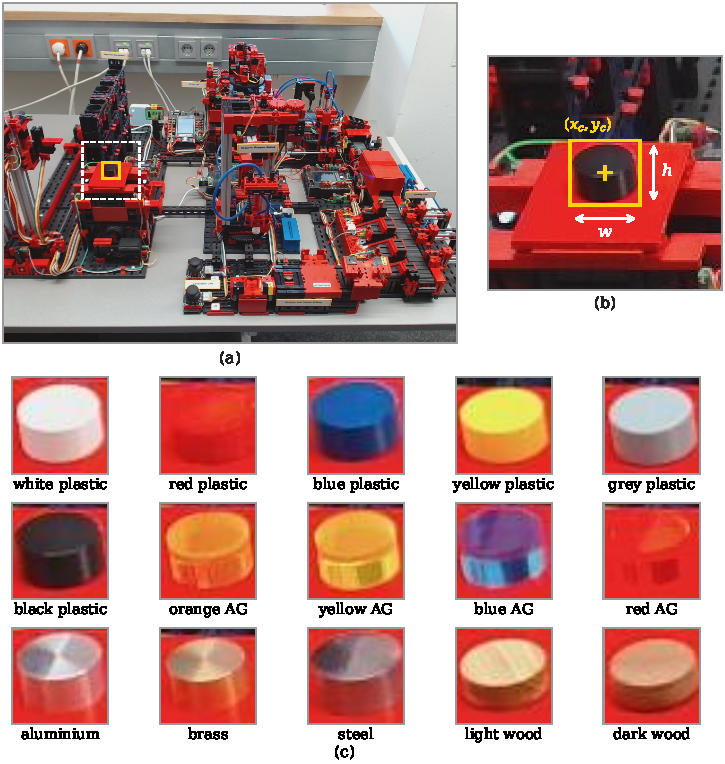
\includegraphics[width=\textwidth]{ch3_figures/fig_ch3_dataset.pdf}
\caption[Learning factory and the 15 workpieces]{Fischertechnik Industry~4.0 learning
factory and the 15 workpieces, where AG is an abbreviation for acrylic glass.
(a) Photograph 2024-04-15-095336 ($960 \times 720$ pixels) with the bounding box of the
black plastic workpiece (yellow) and the enlarged region (white, dashed); (b) enlarged
region with the box centre $(x_c, y_c)$, width $w$ and height $h$ of the label in the
format of the YOLO (You Only Look Once) detector; (c) the 15 workpieces at the same
position, cropped at an object-to-image (O2I) ratio of 90\%. Source of the photographs:
dataset of \cite{schneidereitYOLOv8}.}
\label{fig:bg-dataset}
\end{figure}

\paragraph{Why this dataset}
Four properties make the dataset suitable for the research question. The background
shares colours with several workpieces. Both earlier studies traced detection errors to
such an overlap, the 2023 study for the red workpieces and the 2025 study, with a hedge,
for black plastic among the many black parts of the learning factory
(Section~\ref{sec:related-work-fischertechnik}). Fig.~\ref{fig:bg-dataset}\,(c) shows
the overlap at a single position. Red plastic and red AG almost disappear against the
red plate on which they lie there, and aluminium, steel and grey plastic look much
alike, a similarity that the 2025 study also points out. Aluminium also occurs in the
learning factory itself, which uses it for the supports of the suction
pads~\cite{schneidereitYOLOv8}. These similarities are intended: the 2025 study chose
several workpieces for them, e.g., the black workpiece because it matches the many black
parts of the learning factory. For black plastic, the
workpiece of the real example, the overlap is with the dark parts of the learning
factory rather than with the plate. Since every material was photographed at the same
positions, the models of different materials see the same scenes, and a difference
between them cannot come from a different set of backgrounds. The single box per
photograph allows a crop with a prescribed share of workpiece, which is the variable of
the experiment. Finally, the per-material results of the 2025 study give a reference
point for the material ranking found here, although task and metric differ
(Section~\ref{sec:related-work-fischertechnik}).

\paragraph{Limitation}
Each material is represented by one physical workpiece that was photographed 166 times.
A model can therefore learn properties of that particular piece, e.g., a scratch or the
grain pattern of one piece of wood, together with properties of its material, and the
data cannot separate the two. The results of this thesis describe these 15 workpieces.
Whether they carry over to other workpieces of the same materials is not tested.

% ============================================================================
\subsection{The Object-to-Image Ratio}
\label{sec:background-o2i}

Pawlowski et al.~\cite{pawlowski2019needles} define the O2I ratio by area,

\begin{equation}
r = 100 \cdot \frac{A_{\mathrm{obj}}}{A_{\mathrm{img}}},
\label{eq:bg-o2i}
\end{equation}

where $A_{\mathrm{obj}}$ is the area of the object and $A_{\mathrm{img}}$ the area of
the image, both in pixels, and $r$ is the ratio in percent. This thesis uses the same
definition, with a square crop centred on the box as the image and the area of the
bounding box as the object area. The box also encloses some background around the
cylindrical workpiece, so the workpiece itself covers somewhat less of the crop than
$r$ states. The crop equations and the rule for crops that would extend beyond the
photograph are given in Section~\ref{sec:methodology-crops}.

\paragraph{Area and side length}
Because the ratio is defined by area, it does not fall in proportion to the width of the
object. For a square object of side $s_{\mathrm{obj}}$ in a square image of side
$s_{\mathrm{img}}$, Eq.~\eqref{eq:bg-o2i} gives

\begin{equation}
\frac{s_{\mathrm{obj}}}{s_{\mathrm{img}}} = \sqrt{\frac{r}{100}},
\label{eq:bg-side-fraction}
\end{equation}

where both sides are in pixels and the side fraction on the left is dimensionless. For
the five ratios of this thesis, 90, 70, 50, 30 and 10\%,
Eq.~\eqref{eq:bg-side-fraction} gives 0.95, 0.84, 0.71, 0.55 and 0.32. At 10\%, a square
with the area of the box thus still spans almost a third of the crop width.

\paragraph{A toy scene}
One toy example is used throughout this chapter, small enough that every number can be
checked by hand. Its scene is a grid of $16 \times 16$ grey levels between 0 (black) and
1 (white), shown in Fig.~\ref{fig:bg-o2i}\,(a). A light background of 0.9 stands for the
learning factory, a dark $4 \times 4$ workpiece of 0.1 in the centre stands for black
plastic, and eight dark $2 \times 2$ factory parts of 0.1 are scattered over the
background. Two crops are cut from the same scene. The tight crop is the central
$8 \times 8$ region (Fig.~\ref{fig:bg-o2i}\,(b)). The workpiece covers 16 of its 64
pixels, a ratio of 25\%, and two of the factory parts fall inside it, at the top-left and
bottom-right corners. Since the toy network takes $8 \times 8$ inputs, the tight crop
needs no resizing. The loose crop is the whole scene, in which the workpiece covers
$16/256 = 6.25\%$. It is resized to $8 \times 8$ by averaging blocks of $2 \times 2$
pixels (Fig.~\ref{fig:bg-o2i}\,(c)). The workpiece then occupies $2 \times 2$ pixels,
still $4/64 = 6.25\%$, and every factory part becomes a single pixel. Resizing leaves the
ratio unchanged, but the workpiece has lost half of its width in pixels.

\paragraph{The real crops}
Fig.~\ref{fig:bg-o2i}\,(d) shows the same construction on photograph
2024-04-15-095336. The native crop sides are 36, 42, 48, 62 and 108 pixels at the five
ratios, and every crop is resized to $256 \times 256$ pixels. This photograph is
therefore enlarged about 7 times at 90\% and about 2.4 times at 10\%. At 90\% and 70\%, the crop shows almost only the
workpiece, with a thin strip of red plate and a dark band along the top edge. At 10\%,
the workpiece sits on the red plate of the module, surrounded by red building blocks, a
cable and dark structure.

\begin{figure}[tbp]
\centering
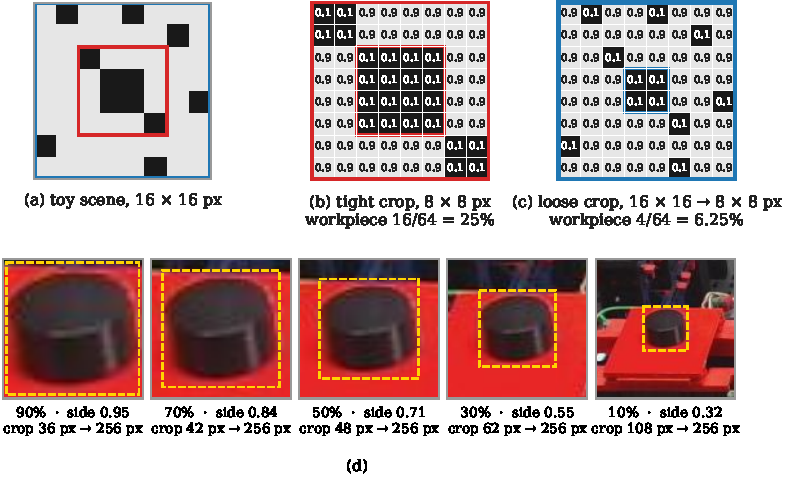
\includegraphics[width=\textwidth]{ch3_figures/fig_ch3_o2i.pdf}
\caption[Object-to-image ratio on the toy scene and on a real photograph]{Object-to-image
(O2I) ratio. (a) Toy scene of $16 \times 16$ pixels with a dark workpiece and dark
factory parts, (red) tight crop, (blue) loose crop; (b) tight crop, $8 \times 8$ pixels;
(c) loose crop, averaged in $2 \times 2$ blocks to $8 \times 8$ pixels; (d) crops of
photograph 2024-04-15-095336 at the five O2I ratios, each resized to $256 \times 256$
pixels, with (dashed) the centred square that has the area of the bounding box, and
below each crop the side fraction $\sqrt{r/100}$ and the native crop side.}
\label{fig:bg-o2i}
\end{figure}

\paragraph{What follows for the thesis}
With a fixed input size, loosening a crop changes two things together. The share of
background in the input grows, and the workpiece covers fewer input pixels. In the toy,
the workpiece shrinks from $4 \times 4$ to $2 \times 2$ pixels. In the real crops, the
side of the square with the area of the box shrinks from about 243 pixels at 90\% to
about 81 pixels at 10\% of the $256$-pixel input. Section~\ref{sec:related-work-o2i}
made this point in contrast to the digit data of Pawlowski et al., who keep the digits
at their native size, and Fig.~\ref{fig:bg-o2i} shows it directly. An effect of the ratio in this thesis
is therefore the combined effect of more background and a smaller workpiece, and the
network of Section~\ref{sec:background-cnn} shows why the second part matters.

% ============================================================================
\subsection{Convolutional Neural Networks}
\label{sec:background-cnn}

Fig.~\ref{fig:bg-cnn-toy} follows the tight toy crop through the first stages of a
convolutional neural network (CNN). A CNN computes a stack of feature maps, each from
the maps before it, and ends in a small number of scores, one per
class~\textbf{[CITATION NEEDED]}.

\paragraph{Convolution}
Let $X \in \mathbb{R}^{C \times N \times N}$ be an input with $C$ channels, e.g., the
three colour channels of a crop or the single grey channel of the toy. A convolutional
layer with $K$ kernels of size $3 \times 3$ computes

\begin{equation}
Y^k_{uv} = b^k + \sum_{q=1}^{C} \sum_{\Delta u=-1}^{1} \sum_{\Delta v=-1}^{1}
W^k_{q,\Delta u,\Delta v}\, X_{q,\,u+\Delta u,\,v+\Delta v}, \qquad k = 1, \dots, K,
\label{eq:bg-conv}
\end{equation}

where $W^k \in \mathbb{R}^{C \times 3 \times 3}$ is the $k$-th kernel with entries
$W^k_{q,\Delta u,\Delta v}$ for the offsets $\Delta u, \Delta v \in \{-1, 0, 1\}$,
$b^k \in \mathbb{R}$ its bias, $(u, v)$ the row and column of an output position, and
$Y^k \in \mathbb{R}^{N \times N}$ the output for kernel $k$. The same kernel is applied at
every position, so a pattern is detected wherever it occurs. Strictly,
Eq.~\eqref{eq:bg-conv} is a cross-correlation, since the kernel is not flipped, but
deep learning calls it a convolution~\textbf{[CITATION NEEDED]}. At the border, the sum
reaches beyond the input. Padding with one row and column of zeros on each side keeps
the output at $N \times N$, which is what the network of this thesis does. The toy
instead repeats the edge pixels, because a border of zeros would look dark to a
detector of dark regions.

The toy network has two kernels. The dark detector has all nine weights equal to $-1/9$
and the bias $+0.6$ (Fig.~\ref{fig:bg-cnn-toy}\,(b)), so its output is 0.6 minus the
mean of the $3 \times 3$ neighbourhood, positive wherever that mean is below 0.6. On the
inside of the workpiece it gives $0.6 - 0.1 = 0.50$, and on open background
$0.6 - 0.9 = -0.30$ (Fig.~\ref{fig:bg-cnn-toy}\,(c)). The light detector has the
weights $+1/9$ and the bias $-0.7$ and responds where the mean is above 0.7.

\paragraph{Rectified linear unit}
The rectified linear unit (ReLU) keeps positive values and sets negative ones to zero,
$A^k = \max(Y^k, 0)$ element by element~\textbf{[CITATION NEEDED]}. The result
$A^k \in \mathbb{R}_{\ge 0}^{N \times N}$ is the feature map of channel $k$.
Fig.~\ref{fig:bg-cnn-toy}\,(d) shows the dark feature map $A^1$ of the tight crop. The
dark detector responds to any dark region that fills its $3 \times 3$ neighbourhood,
whether it belongs to the workpiece or not. Here this is the case at both factory parts,
whose neighbourhoods at the corners of the crop are completed by the repeated border,
and they reach the same 0.50 as the centre of the workpiece. The feature map says where
something dark is, not whether it belongs to the workpiece. This is the situation of
black plastic among the many black parts of the learning factory, with which the 2025
study, with a hedge, explained the difficulty of its detector with this workpiece
(Section~\ref{sec:related-work-fischertechnik}).

\paragraph{Max pooling}
Max pooling with $2 \times 2$ windows halves the resolution by keeping the largest value
of each window~\textbf{[CITATION NEEDED]},

\begin{equation}
M^k_{uv} = \max_{\Delta u,\,\Delta v \in \{0, 1\}} A^k_{2u+\Delta u,\,2v+\Delta v},
\label{eq:bg-maxpool}
\end{equation}

where $M^k \in \mathbb{R}_{\ge 0}^{N/2 \times N/2}$ is the pooled map and $(u, v)$ now
indexes the windows. A response survives pooling if it is the strongest in its window,
and its exact position inside the window is lost. Where several cells of a window share
the maximum, the maximum is not differentiable, and the implementation passes the
gradient to one of them. In the toy, the pooled dark map of
Fig.~\ref{fig:bg-cnn-toy}\,(e) has $4 \times 4$ cells, with 0.50 in the four cells of the
workpiece and in the two corner cells of the factory parts.

\paragraph{From feature maps to a decision}
After the last convolution, the feature maps are summarised into a vector of fixed
length. Adaptive average pooling divides each map into a fixed grid of regions, here
$4 \times 4$, and averages each region. A fully connected layer then computes each of
its outputs as a weighted sum of all its inputs plus a bias. The last layer returns the
logits, real-valued scores without bounds, one per class, which the softmax of
Section~\ref{sec:background-training} turns into probabilities. The toy network instead
takes the mean of each whole pooled map, the special case with a single region, called
global average pooling~\textbf{[CITATION NEEDED]}. This gives
$g = (g_1, g_2) = (0.201, 0.125)$ for the dark and the light channel. A single linear
unit with the weights $(10, -5)$ and no bias then returns the logit
$z = 10 \cdot 0.201 - 5 \cdot 0.125 = 1.39$, and a positive $z$ stands for the decision
``black plastic''. The toy network thus rewards dark regions and penalises light
ones.

\paragraph{Receptive field}
Each value of a feature map depends only on a limited region of the input, its receptive
field~\textbf{[CITATION NEEDED]}. In the toy, one value of $A^1$ sees $3 \times 3$
pixels. Through the four
convolutional layers of the network of this thesis and the three poolings between them,
its width grows as $1 \to 3 \to 4 \to 8 \to 10 \to 18 \to 22 \to 38$ pixels, and the
derivation is given in Section~\ref{sec:methodology-patch}. A unit of the fourth
convolutional layer therefore sees $38 \times 38$ input pixels. The square with the area
of the box spans about 6.4 such widths at 90\% and about 2.1 at 10\%. A pattern detector
of fixed size thus meets a smaller workpiece in a looser crop.

Fig.~\ref{fig:bg-cnn-toy}\,(f) shows what this does to the toy. In the loose crop, the
workpiece covers $2 \times 2$ pixels and no longer fills a $3 \times 3$ neighbourhood.
The dark detector gives only 0.06 on the workpiece itself, and at most 0.14 where a
factory part, now a single pixel, lies diagonally next to it, instead of 0.50 in the
tight crop. The global averages become $g = (0.025, 0.100)$, and the logit falls from
1.39 to $-0.25$. The toy network fails at the small ratio, although the workpiece has not changed. The
toy was built to make this visible, and how strongly the real network is affected cannot
be read from it. It is, however, the scale effect that Section~\ref{sec:methodology-covariates} lists among the
quantities that change together with the ratio.

\begin{figure}[tbp]
\centering
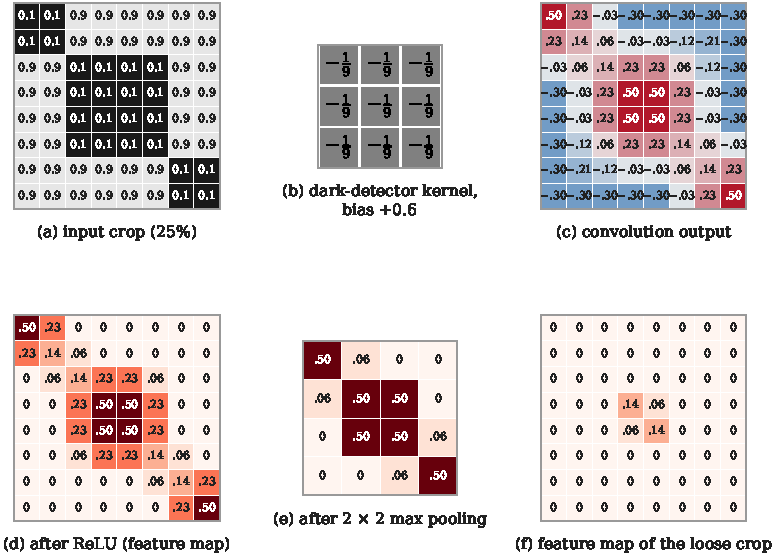
\includegraphics[width=\textwidth]{ch3_figures/fig_ch3_cnn_toy.pdf}
\caption[Building blocks of a CNN on the toy crop]{Building blocks of a convolutional
neural network (CNN) on the toy crop. (a) Grey levels of the tight crop;
(b) $3 \times 3$ kernel of the dark detector, bias $+0.6$; (c) convolution output,
(blue) negative, (red) positive; (d) feature map after the rectified linear unit (ReLU);
(e) after $2 \times 2$ max pooling; (f) feature map of the loose crop of
Fig.~\ref{fig:bg-o2i}\,(c), on the same colour scale as (d).}
\label{fig:bg-cnn-toy}
\end{figure}

\paragraph{The network of this thesis}
All models of this thesis use the network \texttt{MaterialCNN}\-\texttt{Binary}, whose stages are
listed in Tab.~\ref{tab:cnn-architecture}. The toy network is a miniature of it, with one
convolutional layer of two kernels instead of four layers of up to 256, a global
average instead of a $4 \times 4$ grid, and one logit instead of two. Grad-CAM
(Section~\ref{sec:background-gradcam}) is attached to the feature maps of c4 after the
ReLU and before the fourth pooling, i.e., to 256 maps of $32 \times 32$ cells, in the
same place as the toy's maps $A^1$ and $A^2$. Since the adaptive pooling fixes the size
of the vector that enters the fully connected layers, the network accepts inputs of
other sizes, e.g., 128 or 256 pixels, without changes.

\begin{table}[tbp]
\centering
\caption[Architecture of MaterialCNNBinary]{Architecture of \texttt{MaterialCNNBinary}
with the output shape after every stage for a $256 \times 256$ input, given as channels
$\times$ height $\times$ width, where ReLU is the rectified linear unit and Grad-CAM
stands for Gradient-weighted Class Activation Mapping.}
\label{tab:cnn-architecture}
\small
\begin{tabular}{l p{6cm} r}
\hline
\textbf{Stage} & \textbf{Operation} & \textbf{Output shape} \\
\hline
Input & Colour crop (red, green, blue), values in $[0,1]$ & $3 \times 256 \times 256$ \\
c1 & $3 \times 3$ convolution, padding 1, ReLU & $32 \times 256 \times 256$ \\
Pool 1 & $2 \times 2$ max pooling & $32 \times 128 \times 128$ \\
c2 & $3 \times 3$ convolution, padding 1, ReLU & $64 \times 128 \times 128$ \\
Pool 2 & $2 \times 2$ max pooling & $64 \times 64 \times 64$ \\
c3 & $3 \times 3$ convolution, padding 1, ReLU & $128 \times 64 \times 64$ \\
Pool 3 & $2 \times 2$ max pooling & $128 \times 32 \times 32$ \\
c4 & $3 \times 3$ convolution, padding 1, ReLU; & $256 \times 32 \times 32$ \\
 & Grad-CAM attached here (after ReLU, before pooling) & \\
Pool 4 & $2 \times 2$ max pooling & $256 \times 16 \times 16$ \\
Adaptive pooling & Average over a $4 \times 4$ grid of regions & $256 \times 4 \times 4$ \\
Flatten & & 4,096 \\
fc1 & Fully connected, ReLU, dropout 0.5 & 256 \\
fc2 & Fully connected & 2 (logits $z_0, z_1$) \\
\hline
\end{tabular}
\end{table}

\paragraph{Why train from scratch}
The network is trained from randomly initialised weights, as instructed by the
supervisors, and not adapted from a network pre-trained on
ImageNet~\cite{deng2009imagenet}. A network without such priors cannot bring habits
learned on another domain into its decision, e.g., a reliance on typical backgrounds or
the preference for texture over shape that Geirhos et al.~\cite{geirhos2019texture}
found in ImageNet-trained CNNs (Section~\ref{sec:related-work-o2i}). Whatever the models
use, they have learned from the learning factory itself. The price is a small network trained on few images, at most 116 training
photographs per material.

% ============================================================================
\subsection{Training and Evaluating a Binary Classifier}
\label{sec:background-training}

\paragraph{One-vs-rest}
A classification problem with several classes can be split into one binary problem per
class, each of which separates that class from all others~\textbf{[CITATION NEEDED]}.
Here, each binary classifier decides whether a crop shows a given material or one of the
other 14 (Section~\ref{sec:methodology-ovr}), so every binary task is imbalanced by
about 1:14.

\paragraph{Output and loss}
For an input crop $I$, a binary network returns two logits $z_0(I)$ and $z_1(I)$ for the
negative and the positive class. The softmax turns them into
probabilities~\textbf{[CITATION NEEDED]},

\begin{equation}
p_j(I) = \frac{e^{z_j(I)}}{e^{z_0(I)} + e^{z_1(I)}}, \qquad j \in \{0, 1\},
\label{eq:bg-softmax}
\end{equation}

where $p_j(I) \in [0,1]$ and $p_0(I) + p_1(I) = 1$. The predicted class is the one with
the larger logit, which by Eq.~\eqref{eq:bg-softmax} is the class with $p_j > 0.5$; on a
tie the crop is called negative. With two classes, $p_1$ depends only on the difference
of the logits, $p_1 = 1/(1 + e^{-(z_1 - z_0)})$. The single logit $z$ of the toy plays
the role of this difference, so the tight crop with $z = 1.39$ has $p_1 = 0.80$ and is
called positive, and the loose crop with $z = -0.25$ has $p_1 = 0.44$ and is called
negative. During training, the network is penalised for each crop by the
cross-entropy~\textbf{[CITATION NEEDED]},

\begin{equation}
\ell(I, y) = -\log p_y(I),
\label{eq:bg-ce}
\end{equation}

where $y \in \{0, 1\}$ is the true label of the crop and $\ell \ge 0$. The loss is zero
for probability 1 on the true class and grows without bound as that probability
approaches zero. The batch loss $L$ is the mean of $\ell$ of
Eq.~\eqref{eq:bg-ce} over the crops of a batch. Under a strong imbalance, the many
negative crops would dominate this mean, so each crop's loss is multiplied by a weight
that depends on its class and is larger for the rare positive class. The weights used
here and the exact form of the weighted mean are given in
Section~\ref{sec:methodology-training}.

\paragraph{Gradient and backpropagation}
Training changes the parameters $\theta$ of the network, i.e., all kernels, biases and
weights of the fully connected layers, so that the batch loss falls. The gradient
$\nabla_\theta L$, the vector of all partial derivatives of $L$ with respect to the
parameters, points in the direction in which the loss increases fastest. A step of
gradient descent moves against it~\textbf{[CITATION NEEDED]},

\begin{equation}
\theta \leftarrow \theta - \eta\, \nabla_\theta L,
\label{eq:bg-gd}
\end{equation}

where $\eta > 0$ is the learning rate. The network is a chain of functions, layer after
layer, so each partial derivative is a product of local derivatives by the chain rule.
Backpropagation evaluates these products from the output backwards, one layer at a
time~\textbf{[CITATION NEEDED]}. The same computation gives the derivative of a logit
with respect to any intermediate feature map, the quantity on which Grad-CAM is built.

The toy shows how such a derivative is formed. Its logit is $z = 10\,g_1 - 5\,g_2$, the
dark average $g_1$ is the mean of the 16 cells of the pooled map $M^1$, and each cell of
$M^1$ is the maximum of one window of $A^1$ (Eq.~\eqref{eq:bg-maxpool}). By the chain
rule, the derivative of $z$ with respect to one cell of the dark feature map is

\begin{equation}
\frac{\partial z}{\partial A^1_{uv}}
= \frac{\partial z}{\partial g_1} \cdot
  \frac{\partial g_1}{\partial M^1_{u'v'}} \cdot
  \frac{\partial M^1_{u'v'}}{\partial A^1_{uv}}
= 10 \cdot \frac{1}{16} \cdot \delta_{uv},
\label{eq:bg-chain}
\end{equation}

where $(u', v') = (\lfloor u/2 \rfloor, \lfloor v/2 \rfloor)$ is the pooling window that
contains cell $(u, v)$, and $\delta_{uv}$ is 1 if $A^1_{uv}$ is the one cell that max
pooling passes on from that window and 0 otherwise. By Eq.~\eqref{eq:bg-chain}, the
gradient reaches only 16 of the 64 cells of $A^1$, each with $10/16$, and is zero at the
other 48. For the light map, the factor 10 is replaced by $-5$. Raising the dark
response at a cell that wins its window raises the logit. At any other cell, a small
change has no effect. Section~\ref{sec:background-gradcam} averages exactly these
derivatives over the map.

\paragraph{Optimiser and dropout}
Adam is a variant of the step of Eq.~\eqref{eq:bg-gd} that scales the step of each
parameter by running averages of its past gradients and squared
gradients~\textbf{[CITATION NEEDED]}. Dropout sets each output of a layer to zero with a
fixed probability during training and rescales the remaining outputs so that their
expected value is unchanged~\textbf{[CITATION NEEDED]}. A network trained this way is
discouraged from relying on any single unit. Dropout is switched off when the trained
network is evaluated, including during the explainability analyses. The settings used
here are listed in Tab.~\ref{tab:training-config}.

\paragraph{Training, validation and test data}
The parameters are fitted on the training split. After every epoch, i.e., every full pass
over the training split, the model is evaluated on the validation split, and the epoch
with the best validation result is kept. Because the validation split took part in this
choice, its results are slightly optimistic, which matters again for the explainability
analyses, since they also run on validation crops
(Section~\ref{sec:methodology-sampling}). The test split is evaluated once, after all
choices have been made~\textbf{[CITATION NEEDED]}. The split itself is made by
photograph (Section~\ref{sec:methodology-split}).

\paragraph{Metrics under class imbalance}
On a split with true labels, the predictions of a binary classifier fall into four
counts, the true positives $\mathrm{TP}$, false positives $\mathrm{FP}$, false negatives
$\mathrm{FN}$ and true negatives $\mathrm{TN}$. Precision, recall and the F1 score of the
positive class are~\textbf{[CITATION NEEDED]}

\begin{equation}
P = \frac{\mathrm{TP}}{\mathrm{TP} + \mathrm{FP}}, \qquad
R = \frac{\mathrm{TP}}{\mathrm{TP} + \mathrm{FN}}, \qquad
F_1 = \frac{2PR}{P + R},
\label{eq:bg-prf}
\end{equation}

where $P, R, F_1 \in [0,1]$, and a value whose denominator is zero is set to 0. In
Eq.~\eqref{eq:bg-prf}, precision is the part of the crops called positive that are
positive, recall is the part of the positive crops that are found, and $F_1$, their
harmonic mean, is high only if both are. Accuracy is $(\mathrm{TP} + \mathrm{TN})$ divided
by the number of crops. The receiver operating
characteristic (ROC) curve plots the recall against the false positive rate
$\mathrm{FP}/(\mathrm{FP} + \mathrm{TN})$ while the decision threshold on $p_1$ moves
from 1 to 0. The area under this curve (ROC-AUC) equals the probability that a randomly
chosen positive crop receives a higher score than a randomly chosen negative
one~\textbf{[CITATION NEEDED]},

\begin{equation}
\mathrm{AUC} = \Pr\big[p_1(I^+) > p_1(I^-)\big]
+ \tfrac{1}{2} \Pr\big[p_1(I^+) = p_1(I^-)\big],
\label{eq:bg-auc}
\end{equation}

where $I^+$ and $I^-$ are drawn at random from the positive and the negative crops and
$\mathrm{AUC} \in [0,1]$. On a finite split, the probabilities in Eq.~\eqref{eq:bg-auc}
are the fractions of positive--negative pairs that are ordered correctly or tied. A
value of 0.5 corresponds to a random order or a constant score, and 1 to a perfect
ranking. The ROC-AUC thus measures how well the scores rank the crops, independent of a
threshold, while $F_1$ measures the decisions made at the threshold.

Tab.~\ref{tab:bg-toy-metrics} shows why accuracy is not used under the imbalance of this
thesis. Its 30 toy crops have the imbalance 1:14 of the one-vs-rest tasks. The first classifier
always answers ``not X''. The toy model gives the two positive crops the scores 0.9 and 0.7 and the negative crops 0.8, 0.6 and
26 values below 0.5, and calls a crop positive above 0.5. Both reach an accuracy of
$28/30 = 0.933$. The first never finds a positive crop, so its recall and $F_1$ are 0,
and its precision, with a zero denominator, is set to 0. The toy model finds both
positive crops at the cost of two false alarms and reaches $F_1 = 0.667$. Accuracy
cannot tell the two apart, and at 90\% in the real data the ``not X'' answer reaches the
same $1{,}624/1{,}740 = 0.933$ on the training split (Section~\ref{sec:methodology-ovr}).
The thesis therefore reports $F_1$ and ROC-AUC and never accuracy. Of the
$2 \cdot 28 = 56$ positive--negative pairs of the toy model, only one is ordered wrongly, the positive crop at
0.7 below the negative crop at 0.8, so $\mathrm{AUC} = 55/56 = 0.982$. The constant
answer of the first classifier ties every pair and gives 0.5.

\begin{table}[tbp]
\centering
\caption[Metrics of two classifiers on 30 toy crops]{Counts and metrics of two
classifiers on 30 toy crops with 2 positive and 28 negative crops (1:14) at the
threshold 0.5, where TP, FP, FN and TN are the numbers of true positives, false
positives, false negatives and true negatives, Acc., Prec.\ and Rec.\ stand for
accuracy, precision and recall, F1 is the harmonic mean of precision and recall, and
ROC-AUC is the area under the receiver operating characteristic curve.}
\label{tab:bg-toy-metrics}
\small
\setlength{\tabcolsep}{4pt}
\begin{tabular}{lrrrrrrrrr}
\hline
\textbf{Classifier} & \textbf{TP} & \textbf{FP} & \textbf{FN} & \textbf{TN} &
\textbf{Acc.} & \textbf{Prec.} & \textbf{Rec.} & \textbf{F1} & \textbf{ROC-AUC} \\
\hline
Always ``not X'' & 0 & 0 & 2 & 28 & 0.933 & 0.000 & 0.000 & 0.000 & 0.500 \\
Toy model & 2 & 2 & 0 & 26 & 0.933 & 0.500 & 1.000 & 0.667 & 0.982 \\
\hline
\end{tabular}
\end{table}

\paragraph{What the metrics leave open}
$F_1$ and ROC-AUC say how well a model separates its material from the others, but not
which pixels it uses to do so. A model can reach a high $F_1$ by looking at the
workpiece, at the background around it, or at both. The methods of
Sections~\ref{sec:background-occlusion} and~\ref{sec:background-gradcam} ask where the
evidence lies.

% ============================================================================
\subsection{Occlusion Sensitivity}
\label{sec:background-occlusion}

A heatmap, or attribution map, assigns to each region of the input a value for how much
it contributed to a chosen output of the network, here the logit of the positive
class. Methods to compute such maps fall into three families. Perturbation methods
change the input and observe the output. Gradient-based methods read derivatives of the
output inside the network. Relevance propagation passes the output backwards through the
layers and distributes it over the input pixels, as layer-wise relevance propagation
(LRP)~\cite{bach2015lrp, montavon2019lrp} does, the method of the 2025
study~\cite{schneidereitYOLOv8}, which is not used here. Occlusion sensitivity belongs
to the first family, Grad-CAM (Section~\ref{sec:background-gradcam}) to the second.

\paragraph{The method}
Zeiler and Fergus~\cite{zeilerFergus2014} slide a grey patch over the image and record
the output of the network at every patch position. Let $\Omega_{ij}$ be the set of pixels
that the patch covers at position $(i, j)$, and let $I^{(ij)}$ be the crop $I$ with the
fill value written into all channels of the pixels in $\Omega_{ij}$ and unchanged
elsewhere. The occlusion map holds the drop of the target logit,

\begin{equation}
D_{ij} = z(I) - z\big(I^{(ij)}\big), \qquad i, j = 0, \dots, n-1,
\label{eq:bg-occlusion}
\end{equation}

where $z$ is the logit of the target class, $n$ is the number of patch positions per
axis, and $D \in \mathbb{R}^{n \times n}$ is in logit units. A positive $D_{ij}$ means
that covering the region lowered the score, which is read as evidence for the target
class there. A negative $D_{ij}$ means
that covering it raised the score. The map has one value per patch position, so it is
coarser than the input. Zeiler and Fergus recorded the probability of the correct class;
this thesis uses the logit, for the reason given in
Section~\ref{sec:methodology-occlusion-impl}.

\paragraph{Occlusion on the toy}
On the tight toy crop, a grey patch of $2 \times 2$ pixels with the fill value 0.5 is
moved with a stride of 1, which gives $7 \times 7$ positions
(Fig.~\ref{fig:bg-methods-toy}\,(a)). Neighbouring patches overlap by half, as the
$32 \times 32$ patches with stride 16 of the thesis do. The occlusion map of
Eq.~\eqref{eq:bg-occlusion}, shown in Fig.~\ref{fig:bg-methods-toy}\,(b), has its
largest drops over the workpiece, up to 0.44 at its centre, because the grey patch is
lighter than the workpiece and removes dark evidence. A patch over a dark factory part
also gives a clear drop of 0.32. Of the 49 drops, 20 are negative, down to $-0.25$. On
the light background, the grey patch darkens the image. This weakens the light detector,
whose channel the network penalises, and at most of these positions it also
strengthens the dark one, so the score rises. Negative drops are therefore a normal
outcome of occlusion, and how they are treated when a map is summarised is a choice
made in Section~\ref{sec:methodology-normalisation}.

\paragraph{The steel-like crop}
Fig.~\ref{fig:bg-methods-toy}\,(c) shows the tight crop with a workpiece of grey level
0.5, the fill value. The nine patch positions that lie entirely inside the workpiece
replace 0.5 by 0.5, so the input does not change, and their drop in
Fig.~\ref{fig:bg-methods-toy}\,(d) is exactly zero, for this or any other network. The
toy network still responds to the grey workpiece, since 0.5 lies below the threshold of
0.6 of the dark detector, but occlusion cannot detect it. The only positive drops come from
patches over the two factory parts, 0.25 where a patch covers a part entirely and 0.04
where it covers it partly, so occlusion places all positive evidence outside the
workpiece, and the measure of Section~\ref{sec:background-comparison} becomes 0.00. This
is the grey-fill question raised for steel in Section~\ref{sec:related-work-o2i}, in
miniature. The surface of a steel workpiece is grey or reflects grey surroundings, so a
grey patch may remove little of its evidence. For the real steel models, the fill-colour
test of Section~\ref{sec:results-fill} confirms this at 50\%, 30\% and 10\%: with a
black or blurred patch instead of a grey one, occlusion places the evidence of steel on
the workpiece, so its grey-patch result is an artefact of the fill rather than a sign of
background reliance (Section~\ref{sec:discussion-material}).

\paragraph{What occlusion measures}
Occlusion measures what replacing one region alone changes, with everything else left in
place. Its result depends on the fill value, because a region that already resembles
the fill cannot be removed; no fill is neutral for every workpiece, since a black patch,
e.g., removes little of black plastic. It also depends on whether the same evidence is present
elsewhere in the image, since the rest of the image stays visible during each test.

\paragraph{Occlusion on a real crop}
Fig.~\ref{fig:bg-methods-real}\,(a) shows the crop of photograph 2024-04-15-095336 at an
O2I ratio of 70\% with one grey $32 \times 32$ patch and the grid of positions with
stride 16. At this ratio, the margin around the reference square of
Section~\ref{sec:background-comparison} is 21 pixels wide, which holds Grad-CAM cells but
no occlusion patch (Section~\ref{sec:methodology-resolution}). The model is the
black-plastic model trained at 70\%, which classifies the crop as black plastic with
$p_1 > 0.999$ and $z_1 = 6.56$. The $15 \times 15$ map $D$ of
Fig.~\ref{fig:bg-methods-real}\,(b) ranges from $-0.082$ to $+1.111$, and 32 of its 225
drops are negative. The positive drops concentrate on the lower front of the workpiece,
and panel (c) shows them after normalisation and interpolation. The choice of patch
size, stride and fill is justified in Section~\ref{sec:methodology-patch}, and the
results over all models are reported in Section~\ref{sec:results-divergence}.

\begin{figure}[tbp]
\centering
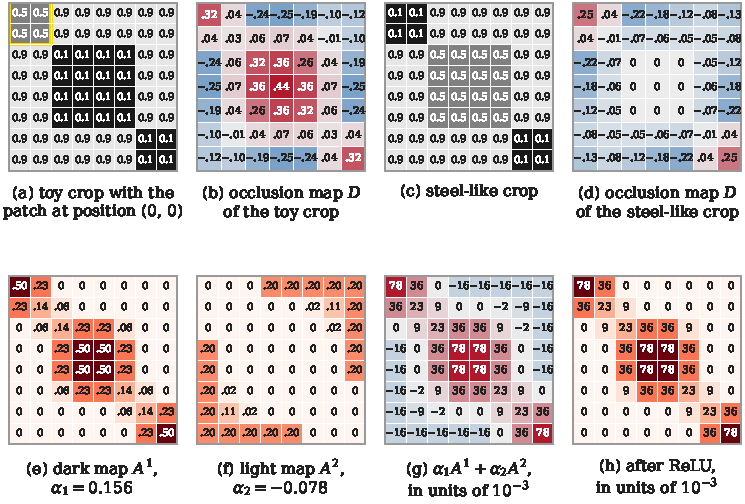
\includegraphics[width=\textwidth]{ch3_figures/fig_ch3_methods_toy.pdf}
\caption[Occlusion sensitivity and Grad-CAM on the toy crop]{Occlusion sensitivity and
Gradient-weighted Class Activation Mapping (Grad-CAM) on the toy crop. (a) Tight crop
with the grey $2 \times 2$ patch at position $(0, 0)$; (b) occlusion map $D$, drop of the
logit per patch position, (blue) negative, (red) positive; (c) steel-like crop,
workpiece at the fill value 0.5; (d) its occlusion map; (e) dark and (f) light feature
map with the Grad-CAM weights $\alpha_1$ and $\alpha_2$; (g) weighted sum of the feature
maps and (h) Grad-CAM map after the rectified linear unit (ReLU), both in units of
$10^{-3}$.}
\label{fig:bg-methods-toy}
\end{figure}

% ============================================================================
\subsection{Grad-CAM}
\label{sec:background-gradcam}

\paragraph{From CAM to Grad-CAM}
Class activation mapping (CAM)~\cite{zhou2016cam} applies to networks whose last feature
maps are globally averaged and fed into a single linear layer. The map of a class is
then the sum of the feature maps, each weighted by its weight in that linear layer, and
shows where the channels that favour the class are active. Gradient-weighted Class
Activation Mapping (Grad-CAM)~\cite{selvaraju2017gradcam} drops this restriction on the
architecture by taking the weights from the gradient. For feature maps
$A^k \in \mathbb{R}_{\ge 0}^{U \times V}$, $k = 1, \dots, K$, of a chosen layer and the
target logit $z$, the weight of channel $k$ is the mean gradient over its map,

\begin{equation}
\alpha_k = \frac{1}{UV} \sum_{u=0}^{U-1} \sum_{v=0}^{V-1}
\frac{\partial z}{\partial A^k_{uv}},
\label{eq:bg-gradcam-weights}
\end{equation}

where $\alpha_k \in \mathbb{R}$ and $U \times V$ is the size of the map. With the weights
of Eq.~\eqref{eq:bg-gradcam-weights}, the Grad-CAM map is the positive part of the
weighted sum of the maps,

\begin{equation}
G = \mathrm{ReLU}\Big( \sum_{k=1}^{K} \alpha_k A^k \Big),
\label{eq:bg-gradcam-map}
\end{equation}

where the ReLU acts element by element and $G \in \mathbb{R}_{\ge 0}^{U \times V}$. A
positive $\alpha_k$ marks a channel whose activity raises the logit on average over the
map, and the ReLU keeps
only the places where such channels outweigh the others. For display and comparison,
$G$ is divided by its maximum. If the weighted sum has no positive entry, $G$ is zero
everywhere and cannot be scaled. How often this happened in the thesis is reported in
Section~\ref{sec:results-degeneracy}. The map has the resolution of the layer it is
attached to. For c4 this is $32 \times 32$, i.e., one cell per 8 pixels of the
$256 \times 256$ input.

\paragraph{Grad-CAM on the toy}
In the toy, Eq.~\eqref{eq:bg-chain} already gives the gradient. The dark map has 16
cells with $10/16$ and 48 with zero, so its mean is
$\alpha_1 = 10/64 = +0.156$. The light map has the factor $-5$ instead of 10, so
$\alpha_2 = -5/64 = -0.078$ (Fig.~\ref{fig:bg-methods-toy}\,(e) and~(f)). The weighted
sum of Fig.~\ref{fig:bg-methods-toy}\,(g) is negative on the light background ring along
the crop border, $-0.078 \cdot 0.20 = -0.016$, and the ReLU sets it to zero
(Fig.~\ref{fig:bg-methods-toy}\,(h)). The map peaks at $0.156 \cdot 0.50 = 0.078$ at the
centre of the workpiece, and equally at the two factory parts. Grad-CAM thus marks every
place where the positively weighted dark channel is active, whether that place is the
workpiece or not. Because the toy has no pooling before its feature maps, the map has
the full $8 \times 8$ resolution of the input.

\paragraph{Where, not what}
Grad-CAM shows where channels with a positive weight are active, not what kind of
feature these channels respond to. A channel that responds to dark regions and one that
responds to a surface texture can look the same in $G$. For aluminium, Grad-CAM places
the evidence on the workpiece at most ratios (Section~\ref{sec:related-work-o2i}), but
the map cannot tell whether the model uses the shape of the workpiece or the texture of
its reflecting surface, the distinction that Geirhos et al.~\cite{geirhos2019texture}
draw for ImageNet-trained CNNs.

\paragraph{Grad-CAM on a real crop}
Fig.~\ref{fig:bg-methods-real}\,(d) shows two of the 256 feature maps of c4 for the crop
at 70\%, $A^{61}$ with $\alpha_{61} = +2.7 \times 10^{-5}$ and $A^{78}$ with
$\alpha_{78} = -4.3 \times 10^{-4}$, the channels that add most to and subtract most from
the weighted sum. Both respond mainly to the red plate around the workpiece and hardly to
the workpiece itself, one with a small positive and the other with a negative weight. Of
the 256 weights, 128 are positive and 128 negative, so the map of
Eq.~\eqref{eq:bg-gradcam-map} is a balance of many channels that push the logit in
opposite directions. The measured $32 \times 32$ map of
Fig.~\ref{fig:bg-methods-real}\,(e) covers the centre and the lower front of the
workpiece, and it marks the dark band along the top edge of the crop, outside the
reference square, only weakly. This is
one image and is meant as an illustration. How the Grad-CAM evidence spreads at 30\% and
10\% is shown in Section~\ref{sec:results-qualitative}. In contrast to occlusion, which
needed 225 separate local tests for the map of panel (b), Grad-CAM reads all feature
maps at once in one forward and one backward pass.

\begin{figure}[tbp]
\centering
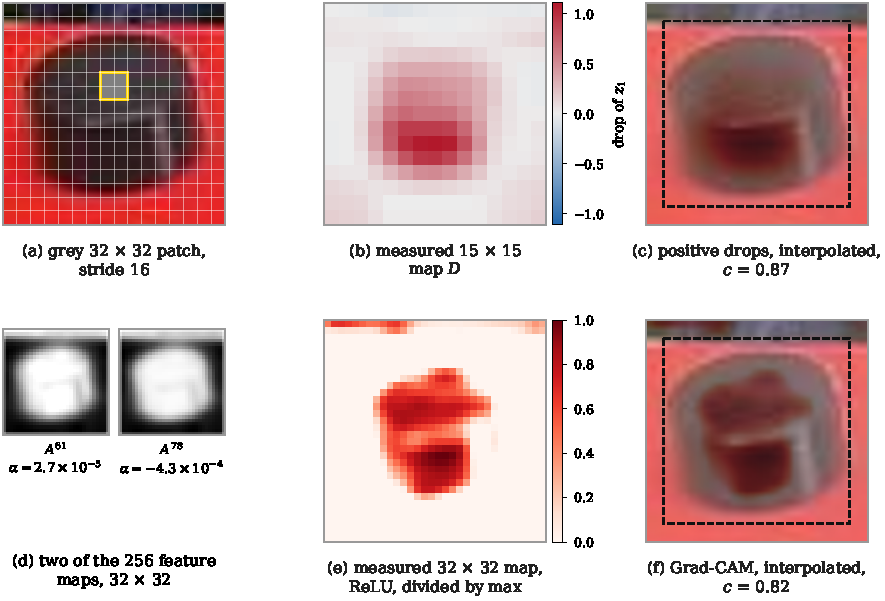
\includegraphics[width=\textwidth]{ch3_figures/fig_ch3_methods_real.pdf}
\caption[Occlusion sensitivity and Grad-CAM on one real crop]{Occlusion sensitivity and
Gradient-weighted Class Activation Mapping (Grad-CAM) for one crop of black plastic at
an object-to-image (O2I) ratio of 70\% (photograph 2024-04-15-095336) and the 70\%
black-plastic model. (a) Crop with one grey $32 \times 32$ patch and the stride-16 grid;
(b) measured $15 \times 15$ map $D$ of drops of the positive-class logit $z_1$;
(c) positive drops, normalised and bilinearly interpolated for display, with the
reference square (dashed) and the centre measure $c$; (d) two of the 256 feature maps
of the fourth convolutional layer, $32 \times 32$, with their weights $\alpha$ (dark
for high activation);
(e) measured $32 \times 32$ Grad-CAM map after the rectified linear unit (ReLU),
divided by its maximum; (f) Grad-CAM, interpolated for display, with $c$. The smooth
appearance of (c) and (f) comes from the interpolation, not from the measurement.}
\label{fig:bg-methods-real}
\end{figure}

% ============================================================================
\subsection{Object versus Background in a Heatmap}
\label{sec:background-comparison}

The research question asks whether the evidence of a model lies on the workpiece or on
the background. For one heatmap, this becomes the question whether the map favours the
workpiece. Since every crop is centred on its box, the workpiece is approximated by a
centred reference square with the area of the box, the dashed square in
Fig.~\ref{fig:bg-o2i}\,(d). Two summaries of a map suggest themselves. The first is the
share of the summed map that lies inside the square. The second compares the mean
importance per pixel inside the square with that outside it.

\paragraph{Why per pixel}
Fig.~\ref{fig:bg-centre-toy} applies both summaries to the toy. A flat map, with the same
value everywhere, has no preference for either region. Its share inside the square
equals the area of the square, 0.25 for the tight crop and 0.06 for the loose one
(panels (a) and (b)), so the share of a map without any preference changes with the
ratio. Its mean per pixel is the same inside and outside, and the per-pixel comparison
gives 0.50 for any square. Only the per-pixel version thus has a fixed level for ``no
preference''. This thesis therefore uses the per-pixel comparison and calls it the
centre measure $c$. It is defined exactly in Eq.~\eqref{eq:center-frac}
(Section~\ref{sec:methodology-centerfrac}). Values above 0.5 mean that a pixel inside the
square carries more importance on average than a pixel outside it, and values below 0.5
the reverse.

The toy maps of panels (c) and (d) both favour the workpiece. For occlusion, only the
positive drops are kept, each pixel receives the mean of the positive drops of the
patches that cover it, and the map is divided by its maximum. This gives $c = 0.83$. The Grad-CAM map divided by its
maximum gives $c = 0.84$. A pixel inside the square is thus about 4.9 and 5.2 times as
important as a pixel outside it. The shares of 0.62 and 0.64 are lower, because the
square covers only a quarter of the crop. For the real crop of
Fig.~\ref{fig:bg-methods-real}, $c$ is 0.87 for the positive occlusion drops and 0.82 for
Grad-CAM. The slightly lower Grad-CAM value seems to come from its weak response along
the dark band at the top edge, which lies outside the square. At this ratio, however, no occlusion patch lies
entirely outside the square, so the two values are not fully comparable
(Section~\ref{sec:methodology-resolution}).

\begin{figure}[tbp]
\centering
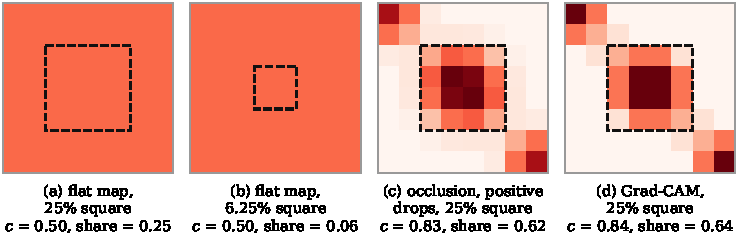
\includegraphics[width=\textwidth]{ch3_figures/fig_ch3_centre_measure_toy.pdf}
\caption[Comparing importance inside and outside a centred square on the
toy]{Comparing importance inside and outside a centred square on the toy, where $c$ is
the centre measure and share is the part of the summed map inside the square (dashed).
(a, b) Flat map with the square of the tight and of the loose crop; (c) occlusion map
with positive drops only, each pixel the mean of the positive drops of the patches that
cover it, divided by its maximum; (d) Grad-CAM map divided by its maximum, where Grad-CAM stands for
Gradient-weighted Class Activation Mapping.}
\label{fig:bg-centre-toy}
\end{figure}

\paragraph{Why the two methods can disagree}
Occlusion and Grad-CAM answer different questions. Occlusion asks what replacing one
patch with grey changes in the score while the rest of the image stays in place.
Grad-CAM asks where the channels that push the score up are active. Both can be right
about their own question and still point to different regions, and neither map is
ground truth for what the model uses~\textbf{[CITATION NEEDED]}. One way in which the
two answers could separate is a hypothesis that this thesis cannot test directly. If the
background contains many similar cues, like a room full of clocks, covering one of them
leaves the others visible and changes the score little, while Grad-CAM marks all of
them at once.

The toy does not show such a divergence. Its two maps agree, with $c = 0.83$ and 0.84.
What it shows are the ingredients. Both methods mark the dark factory parts, but for
different reasons: Grad-CAM because the dark channel is active there, occlusion because
covering them lowers the score. In the toy the two reasons coincide, but nothing forces
them to. Occlusion also depends on the fill, and for the steel-like crop it
places all positive evidence outside the workpiece. Its drops can be negative, so the
treatment of negative values enters the summary.

Other questions the toy cannot settle at all. Its patch is chosen to fit its workpiece,
its maps are read without interpolation, and its square is exactly the workpiece. The
real crops have none of these conveniences: 75 models at five ratios, patches on a
$256 \times 256$ input, coarse maps that must be brought to the pixel grid, and a
square that only approximates a box that itself encloses some background. Before values
of $c$ can be compared across materials and ratios, each of these needs a fixed and
justified setting, and Section~\ref{sec:methodology} provides them.

% !TEX root = ../main.tex
\section{Methodology}
\label{sec:methodology}

\subsection{Dataset Preparation and Crop Extraction}
\label{sec:methodology-crops}

The original dataset provides one bounding box per image, marking the workpiece's
location and size. To study how classification behaviour changes as the object occupies
more or less of the frame, this thesis defines the \emph{object-to-image (O2I) ratio} as
the fraction of a cropped image's \emph{area} occupied by the object's bounding box, and
generates, for every image, a square crop centred on the bounding box centre such that the
object occupies a chosen target ratio of the crop's area. For a bounding box of pixel
width $w$ and height $h$, the side length of the crop achieving a target ratio $r$ is

\begin{equation}
\text{crop\_side} = \sqrt{\frac{w \times h}{r}}.
\label{eq:crop-side}
\end{equation}

Five target ratios were used: $90\%$, $70\%$, $50\%$, $30\%$, and $10\%$, evenly spaced
from almost-pure-object to object-dominated-by-background. This range and spacing was
chosen to give a readable ratio-vs-performance curve with enough points to distinguish a
gradual decline from a sudden cliff, while keeping the number of required training runs
manageable; a $10\%$ floor was used to avoid the object shrinking to only a handful of
pixels after resizing to the network's input resolution. Applying this procedure to all 15
materials at all 5 ratios yields $15 \times 5 = 75$ distinct sub-datasets, each internally
consistent (same camera, same background, same object, only the crop tightness differs).

\subsection{Experimental Design: One-vs-Rest Binary Classification}
\label{sec:methodology-ovr}

An initial design trained a single 15-class classifier per ratio (5 models total, one per
ratio, each choosing among all 15 materials). This thesis instead adopts a
\emph{one-vs-rest} design: for every (material, ratio) combination, a separate binary
classifier is trained to answer the narrower question ``is this crop material $X$, or not''
(target $=1$ for the material in question, target $=0$ for crops of any of the other 14
materials at that ratio). This produces $15 \times 5 = 75$ independent binary models in
total.

This reformulation was adopted because it lets each material's sensitivity to the O2I
ratio be read off directly and independently: with one detector per material, the
detectability of e.g.\ aluminium as the object shrinks can be tracked in isolation, rather
than being entangled with how the other 14 materials' decision boundaries happen to shift
in a shared 15-way classifier. Every one-vs-rest model uses the same fixed random seed
($42$) on every run, so that seed variation is never a confound when comparing across
materials or ratios -- the ratio (and, for a given run, the material) is the only thing
that changes between models.

\subsection{Training Configuration}
\label{sec:methodology-training}

All 75 models share an identical training configuration, summarised in
Table~\ref{tab:training-config}.

\begin{table}[h]
\centering
\begin{tabular}{lp{9cm}}
\hline
\textbf{Parameter} & \textbf{Value} \\
\hline
Input resolution & $256 \times 256$ \\
Epochs & 100 (primary); 200 for a supplementary check, Section~\ref{sec:results-200epoch} \\
Batch size & 16--32 \\
Optimiser & Adam \\
Random seed & 42 (fixed across every run) \\
Loss & Weighted binary cross-entropy (see below) \\
\hline
\end{tabular}
\caption{Training configuration used for every one-vs-rest model.}
\label{tab:training-config}
\end{table}

An earlier, smaller-scale comparison on the original 15-class design had found
$128\times128$ input crops to perform marginally better than $256\times256$ ($80.5\%$ vs.\
$79.5\%$ validation accuracy at 25 epochs) while training $2.4\times$ faster, and $128px$
was initially adopted on that basis. For the one-vs-rest redesign, the input resolution
was changed to $256\times256$; this required no architecture change, since the adaptive
average pooling layer described in Section~\ref{sec:background-cnn} makes
\texttt{MaterialCNN} input-size independent by construction.

\subsubsection{Why Accuracy Is Not a Meaningful Metric Here}
\label{sec:methodology-metrics}

Reformulating the problem as 75 binary one-vs-rest tasks has an important side effect:
every task now has a severe class imbalance, since each binary classifier sees roughly one
positive example (the target material) for every 14 negative examples (all other
materials), an imbalance of approximately $1{:}14$. Under this imbalance, plain accuracy
is not a meaningful metric: a trivial classifier that always predicts ``not the target
material,'' without having learned anything about the visual difference between materials,
already achieves roughly $93\%$ accuracy by construction. This was verified directly on
synthetic data reproducing the class balance: the always-negative baseline scored $93.3\%$
accuracy while its F1 score -- which specifically measures how well the positive
(target-material) class is identified -- was $0.000$.

To avoid this failure mode, three changes were made to the training and evaluation
procedure, all three of which are applied together on every run:
\begin{enumerate}
\item \textbf{Weighted loss.} The loss function upweights the minority (positive) class by
approximately $14\times$, roughly matching the class imbalance ratio, so that misclassifying
a true positive is penalised proportionally more than misclassifying a true negative.
\item \textbf{F1 and ROC-AUC as the reported metrics.} Accuracy is never reported for any
one-vs-rest result in this thesis; F1 score and ROC-AUC on the positive (target-material)
class are used throughout instead, since both remain informative under class imbalance.
\item \textbf{Best-epoch checkpointing by F1, not accuracy.} The model checkpoint saved for
each run is the epoch with the highest validation F1 score, rather than the epoch with the
highest validation accuracy, so that the saved model is the one that is actually best at
the task that matters.
\end{enumerate}

\subsubsection{Validation and Test Split Protocol}
\label{sec:methodology-split}

All model development, hyperparameter decisions, and epoch selection were performed using
a held-out validation split. The test split was set aside at the start of the project and
was not inspected or used for any decision-making during development; it is reserved
exclusively for the final, once-only reported evaluation, so that no reported number is
the product of repeated tuning against the same data it is evaluated on.

\subsection{Explainability Pipeline}
\label{sec:methodology-explainability}

Both occlusion sensitivity (Section~\ref{sec:background-occlusion}) and Grad-CAM
(Section~\ref{sec:background-gradcam}) were implemented against the trained one-vs-rest
models and applied consistently across all 75 (material, ratio) combinations.

\subsubsection{Occlusion Sensitivity: Implementation and a Methodological Correction}
\label{sec:methodology-occlusion-impl}

The implementation slides a $32\times32$ grey patch across each $256\times256$ input
image with a stride of 16 pixels, re-running the trained model at every patch position and
recording the change in the network's output for the target class relative to the
unoccluded image. This produces a coarse $15\times15$ grid of importance values, which is
then upsampled by interpolation to the full $256\times256$ resolution to form the final
heatmap.

This specific patch size and stride were not tuned empirically against alternatives, so it
is worth stating explicitly why they are a reasonable choice rather than an arbitrary one.
Four considerations motivate the $32\times32$/stride-16 configuration. First,
\emph{computational cost}: a stride of 16 over a $256\times256$ image yields
$\left(\frac{256-32}{16}+1\right)^2 = 15^2 = 225$ patch positions, and therefore 225
forward passes per image. A stride of 1 would require $225^2 \approx 50{,}625$ forward
passes per image -- more than two hundred times as many -- which is infeasible at the
scale used in this thesis (75 models $\times$ 10 sampled images per method,
Section~\ref{sec:methodology-centerfrac}). A stride of half the patch size (16 is half of
32) is a standard compromise: adjacent patches overlap by 50\%, which smooths the
resulting heatmap after upsampling, without the cost of a finer stride. Second,
\emph{scale relative to the network's own receptive field}: the CNN backbone
(Table~\ref{tab:cnn-architecture}) halves spatial resolution at each of its four
pooling stages ($256\to128\to64\to32\to16$), so a single unit in the final feature map
used by Grad-CAM already aggregates information from a neighbourhood on the order of
tens of input pixels. A $32\times32$ occlusion patch is comparable to this scale, meaning
a single occluded patch is capable of meaningfully perturbing the activations the network
itself treats as one local unit of evidence, rather than being small enough to disappear
into the receptive field of a single feature or large enough to blur together several
unrelated ones. Third, \emph{scale relative to the object across the studied O2I ratios}:
at the smallest ratio studied (10\%), the object occupies a square of side
$\sqrt{0.10}\times256\approx81$ pixels (Equation~\ref{eq:crop-side}), so a $32\times32$
patch covers under half of the object's width -- large enough to register a meaningful
occlusion, small enough that several patches are needed to cover the object fully, which
is what gives the heatmap genuine spatial resolution \emph{within} the object rather than
one patch swallowing it whole. At the largest ratio (90\%), the same patch is a small
fraction of the object, allowing the heatmap to resolve structure across both object and
background. Fourth, \emph{consistency with Grad-CAM}: the Grad-CAM heatmap
(Section~\ref{sec:methodology-gradcam-impl}) is itself produced at $32\times32$ resolution
before upsampling, so the two methods are compared at a matched spatial resolution rather
than one being systematically coarser than the other. Together these considerations were
judged sufficient to justify the configuration used throughout this thesis; they are not a
substitute for an empirical sweep over patch sizes, which remains a possible direction for
future work (Section~\ref{sec:discussion-future}) but was not carried out here.

An important implementation decision, discovered during initial testing rather than
assumed in advance, concerns exactly which network output is measured. The first
implementation measured the change in the model's \emph{softmax probability} for the
target class. On a confidently and correctly classified test image, this produced a
heatmap that was completely flat -- minimum, maximum, and mean all exactly $0.0$ -- even
though Grad-CAM, run on the same model and image, produced a clear and sensible heatmap.
The cause was diagnosed rather than assumed: softmax probability is bounded to the
interval $[0, 1]$, and for a sufficiently confident model, the probability for the correct
class rounds to exactly $1.0$ in 32-bit floating-point representation both before and
after occluding any single patch, so the measured difference is always $1.0 - 1.0 = 0.0$
regardless of how much the model's underlying evidence actually changes. The fix was to
measure the change in the raw \emph{logit} (the network's output before the softmax
nonlinearity is applied) instead of the probability. Because logits are unbounded, they do
not saturate this way; on the same model and image, the logit-based heatmap ranged from
$-2.405$ to $3.145$ with clear, interpretable structure (strongest on a reflective rim and
a highlight on the object itself). \textbf{Every occlusion sensitivity result reported in
this thesis (Section~\ref{sec:results}) is therefore computed on the raw logit, not the
softmax probability}, specifically to avoid this saturation failure mode on confidently
trained classifiers.

\subsubsection{Grad-CAM: Implementation}
\label{sec:methodology-gradcam-impl}

The Grad-CAM implementation attaches to the final $256$-channel convolutional feature map
identified in Table~\ref{tab:cnn-architecture}. For a given input image and target class,
one forward pass computes this feature map and the class score; one backward pass computes
the gradient of that score with respect to every unit of the feature map. The gradients
are globally average-pooled within each of the 256 channels to obtain one importance
weight per channel; the channels are combined into a single $32\times32$ map using these
weights, passed through a ReLU (retaining only positive contributions to the target
class), min-max normalised, and upsampled to $256\times256$ to match the input resolution.

\subsubsection{The \texorpdfstring{$\text{center\_frac}$}{center\_frac} Metric}
\label{sec:methodology-centerfrac}

To compare occlusion sensitivity and Grad-CAM quantitatively, rather than only visually,
each heatmap is reduced to a single number, $\text{center\_frac}$: the fraction of the
heatmap's total (min-max normalised) importance that falls inside a square box centred on
the image, sized so that the box's \emph{area} equals that image's O2I ratio,

\begin{equation}
\text{box\_side} = \sqrt{\frac{\text{ratio}}{100}} \times 256,
\label{eq:box-side}
\end{equation}

matching the same area-based ratio definition used for crop generation
(Equation~\ref{eq:crop-side}). A $\text{center\_frac}$ of $1.0$ means the heatmap's
importance is entirely concentrated inside the (ratio-sized) central box, i.e.\ fully
object-focused; a value of $0.0$ means it falls entirely outside, i.e.\ fully
background-focused. For the rare case of a completely flat heatmap (denominator
approximately zero, see Section~\ref{sec:results-robustness}), a neutral fallback value of
$0.5$ is used rather than an undefined ratio. For each of the 75 models, $\text{center\_frac}$
is computed for both methods on 10 sampled validation images per model (fixed seed 42, so
sampling is reproducible), giving $75 \times 10 = 750$ image analyses per method.

% !TEX root = ../main.tex
\section{Experiments and Results}
\label{sec:results}

\subsection{Training Completion and a Data-Integrity Check}
\label{sec:results-training}

All 75 one-vs-rest models (Section~\ref{sec:methodology-ovr}) were trained to completion
on an NVIDIA RTX A6000 (48\,GB), with the 48 models still genuinely requiring training at
the start of the final training session finishing in $144.4$ minutes.

Before accepting the trained model count as correct, an automated ``resume'' check (which
determines whether a given (material, ratio) model still needs training by checking
whether an output folder already exists for it) reported that 29 of the 75 models were
already complete. This count was verified rather than trusted at face value: two of the
``complete'' folders contained F1/AUC values identical to an earlier 3-epoch smoke test
used only to confirm the pipeline ran end-to-end, which was too exact a match to be
coincidental. Checking the actual recorded epoch count in every folder's training log
confirmed that these two folders held only 3 epochs of training, not 100, and that a
third model had never been started at all. The resume check's file-existence test could
not distinguish a genuine 100-epoch run from a leftover partial run that happened to write
output to the same location. The true state was $27/75$ genuinely complete, not 29; the
affected folders were deleted and retrained under the full configuration before any result
in this thesis was recorded. This is reported here as a data-integrity check on the
reported results, not merely a debugging anecdote: every F1/AUC value in this thesis
reflects a full, verified 100-epoch run.

\subsubsection{Convergence Behaviour: A Training-Dynamics Sanity Check}
\label{sec:results-convergence}

Before reporting final classification performance, the training and validation loss
curves recorded for every model were inspected directly, rather than trusting the
recorded ``best epoch'' F1 score in isolation. Figure~\ref{fig:loss-curves} shows these
curves for all 15 materials at the $90\%$ O2I ratio, over the full 100 training epochs.

\begin{figure}[h]
\centering
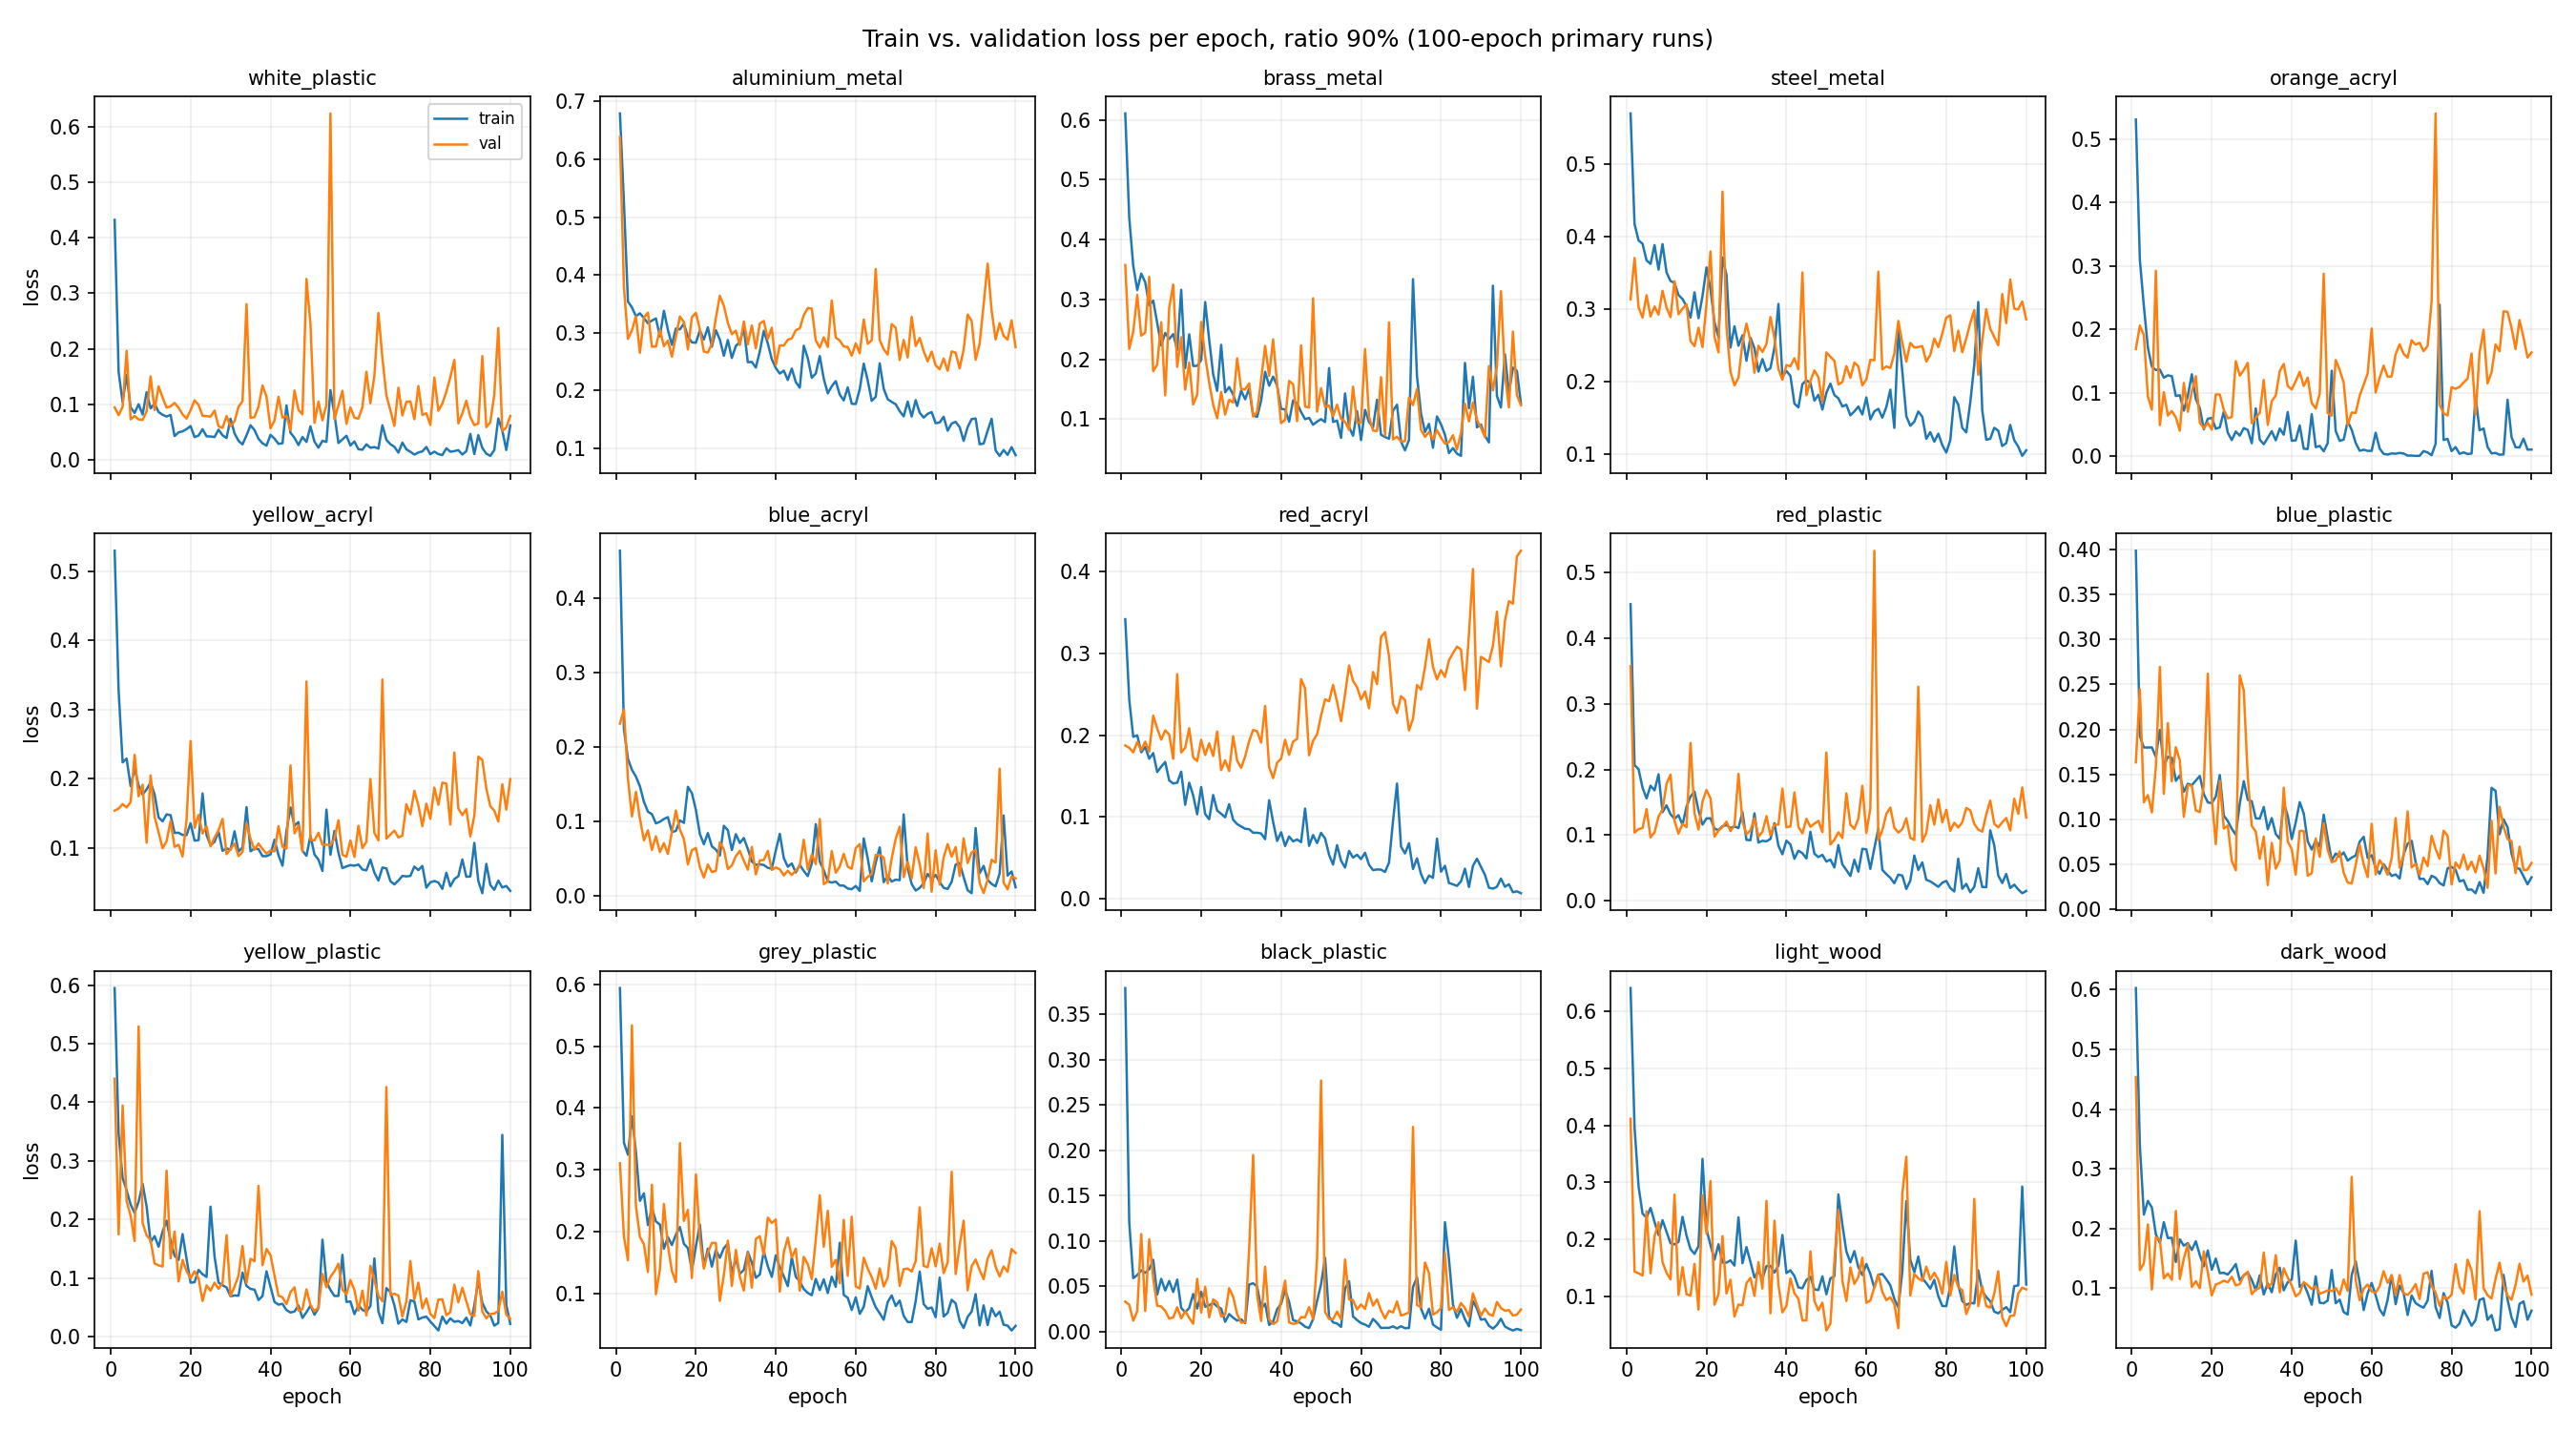
\includegraphics[width=\textwidth]{fig_loss_curves_ratio90.png}
\caption{Training (blue) and validation (orange) loss per epoch, for all 15 materials at
the $90\%$ O2I ratio, over the full 100-epoch primary training run. Validation loss is
visibly noisier than training loss throughout, consistent with the smaller size of the
validation split relative to the training split.}
\label{fig:loss-curves}
\end{figure}

Most materials show the expected pattern for a network trained from scratch (i.e.\ without
an ImageNet-pretrained head start, per the supervisor's instruction,
Section~\ref{sec:methodology-training}): a rapid initial drop in both losses over the
first $5$--$10$ epochs, followed by a slower, noisy decline, with validation loss
consistently above and noisier than training loss but not diverging from it. Black
plastic and brass metal show the cleanest, most stable convergence of the 15, with both
curves settling to a low, stable value by roughly epoch 40. Red acryl is the clearest
counter-example: its training loss continues falling smoothly toward zero across all 100
epochs, but its validation loss reaches a minimum around epoch 20--30 and then rises
steadily for the remainder of training, ending roughly twice as high as its minimum --
textbook overfitting, where the network increasingly memorises training-specific detail
that does not generalise to unseen validation crops. This is precisely the failure mode
that the project's F1-based checkpointing strategy (\texttt{BEST\_METRIC = "f1"},
Section~\ref{sec:methodology-training}) is designed to guard against: rather than using
the final epoch's weights, training keeps the checkpoint from whichever epoch achieved the
best validation F1 score, which for red acryl falls well before this later overfitting
sets in. Inspecting these curves therefore serves two purposes at once: it confirms that
no model's reported result was undermined by a training run that diverged or failed to
converge, and it demonstrates concretely, on a real example, why checkpoint selection by
validation F1 rather than by final epoch was the correct design choice for a
from-scratch, non-pretrained CNN.

\subsubsection{Primary Result: Test-Set F1 by Material and O2I Ratio}
\label{sec:results-primary-table}

Every number reported up to this point in the thesis -- including every F1 score used for
checkpoint selection during training -- was computed on the \emph{validation} split, which
is correct and expected during development (Section~\ref{sec:methodology-split}), but
means that no number reported so far is a final, once-touched measure of how well these
models actually generalise. Following the project's locked protocol, the test split was
therefore touched exactly once, at this point, purely to compute final performance: each
of the 75 trained checkpoints was loaded and evaluated, in inference only (no further
training, no further decisions made on the basis of the result), on its corresponding
held-out test crops. Table~\ref{tab:ovr-full-results} reports the resulting test-set F1
score for every (material, ratio) combination -- the primary quantitative result of Phase
2 of this thesis.

\begin{table}[h]
\centering
\footnotesize
\begin{tabular}{lccccc}
\hline
\textbf{Material} & \textbf{90\%} & \textbf{70\%} & \textbf{50\%} & \textbf{30\%} & \textbf{10\%} \\
\hline
White plastic   & 0.94 & 0.87 & 0.86 & 0.81 & 0.88 \\
Aluminium metal & 0.61 & 0.59 & 0.51 & 0.33 & 0.39 \\
Brass metal     & 0.91 & 0.85 & 0.84 & 0.94 & 0.77 \\
Steel metal     & 0.52 & 0.47 & 0.56 & 0.53 & 0.29 \\
Orange acryl    & 0.82 & 0.89 & 0.81 & 0.73 & 0.76 \\
Yellow acryl    & 0.79 & 0.87 & 0.85 & 0.78 & 0.69 \\
Blue acryl      & 0.96 & 0.98 & 0.94 & 0.96 & 0.91 \\
Red acryl       & 0.79 & 0.75 & 0.74 & 0.64 & 0.64 \\
Red plastic     & 0.85 & 0.83 & 0.70 & 0.71 & 0.65 \\
Blue plastic    & 0.94 & 0.96 & 0.90 & 0.92 & 0.82 \\
Yellow plastic  & 0.88 & 0.86 & 0.94 & 0.91 & 0.89 \\
Grey plastic    & 0.77 & 0.82 & 0.70 & 0.74 & 0.64 \\
Black plastic   & 0.90 & 0.96 & 0.96 & 0.96 & 0.94 \\
Light wood      & 0.78 & 0.71 & 0.83 & 0.74 & 0.73 \\
Dark wood       & 0.84 & 0.81 & 0.81 & 0.83 & 0.82 \\
\hline
\textbf{Mean} & \textbf{0.820} & \textbf{0.816} & \textbf{0.796} & \textbf{0.769} & \textbf{0.720} \\
\hline
\end{tabular}
\caption{Test-set F1 score for all 75 one-vs-rest models (15 materials $\times$ 5 O2I
ratios), computed once, after training, on the held-out test split. The bottom row is the
mean across all 15 materials at each ratio.}
\label{tab:ovr-full-results}
\end{table}

The mean F1 score across all 15 materials declines monotonically and, notably,
\emph{accelerates} as the O2I ratio shrinks: from $0.820$ at a $90\%$ ratio, the mean falls
only slightly to $0.816$ at $70\%$ and $0.796$ at $50\%$, before dropping more steeply to
$0.769$ at $30\%$ and $0.720$ at $10\%$. Taken at face value, this is already a direct,
classification-level answer to part of the thesis's research question: shrinking the
object relative to the frame measurably degrades classification accuracy, and the
complex factory background is the only thing left to fill the remaining space, so this
decline is consistent with the background increasingly interfering with classification
as the object shrinks. Figure~\ref{fig:f1-per-material} and Figure~\ref{fig:f1-heatmap}
visualise this same result in two complementary ways.

\begin{figure}[h]
\centering
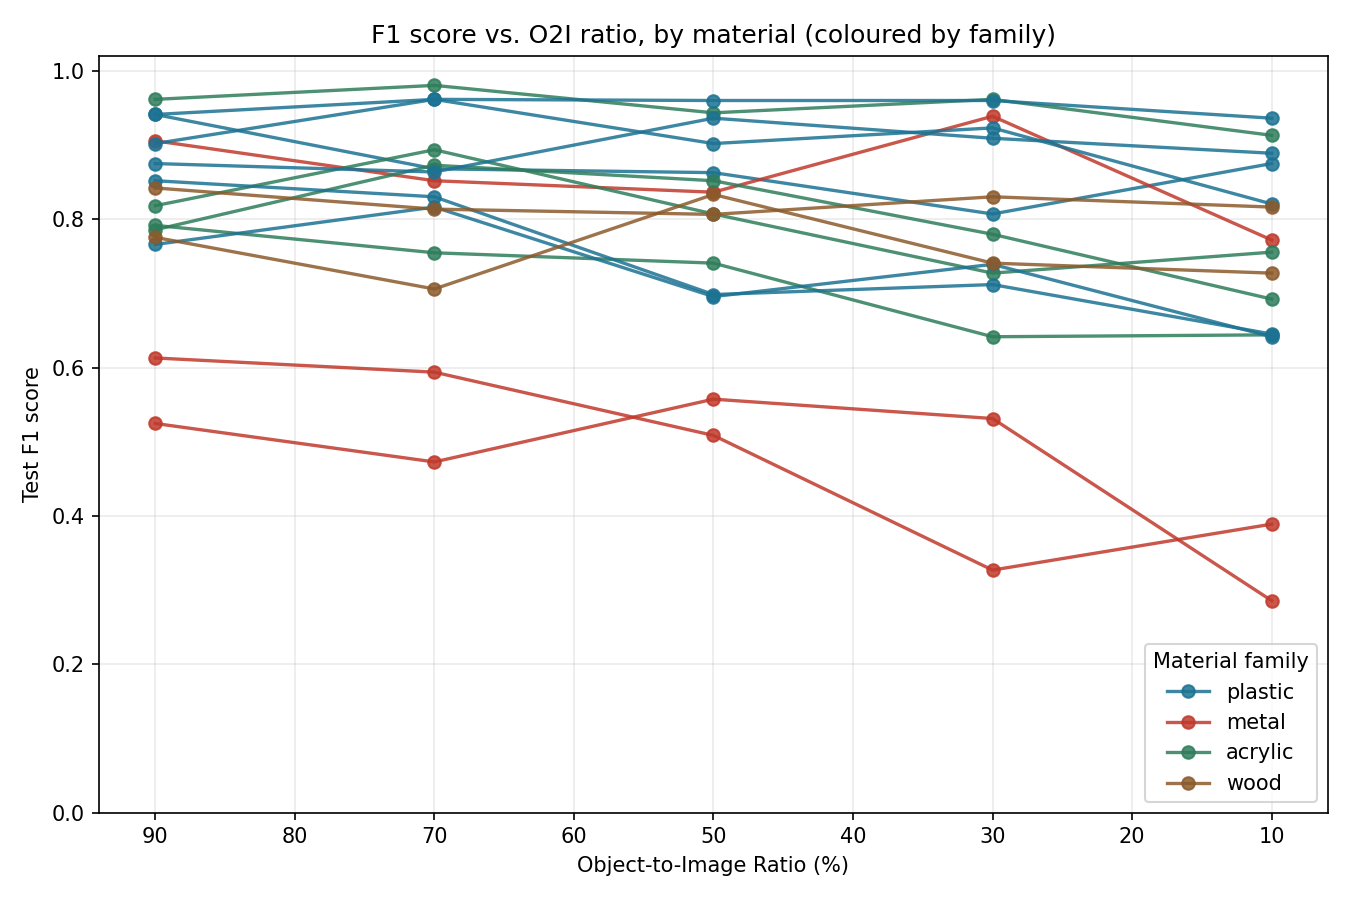
\includegraphics[width=0.85\textwidth]{fig_f1_per_material.png}
\caption{Test F1 score against O2I ratio for all 15 materials, coloured by material
family (plastic, metal, acrylic, wood). Most materials cluster in a band between roughly
$0.7$ and $0.95$ F1 with a gentle downward slope; the two bare, reflective metals
(aluminium, steel; red) are visibly separated below this band at every ratio.}
\label{fig:f1-per-material}
\end{figure}

\begin{figure}[h]
\centering
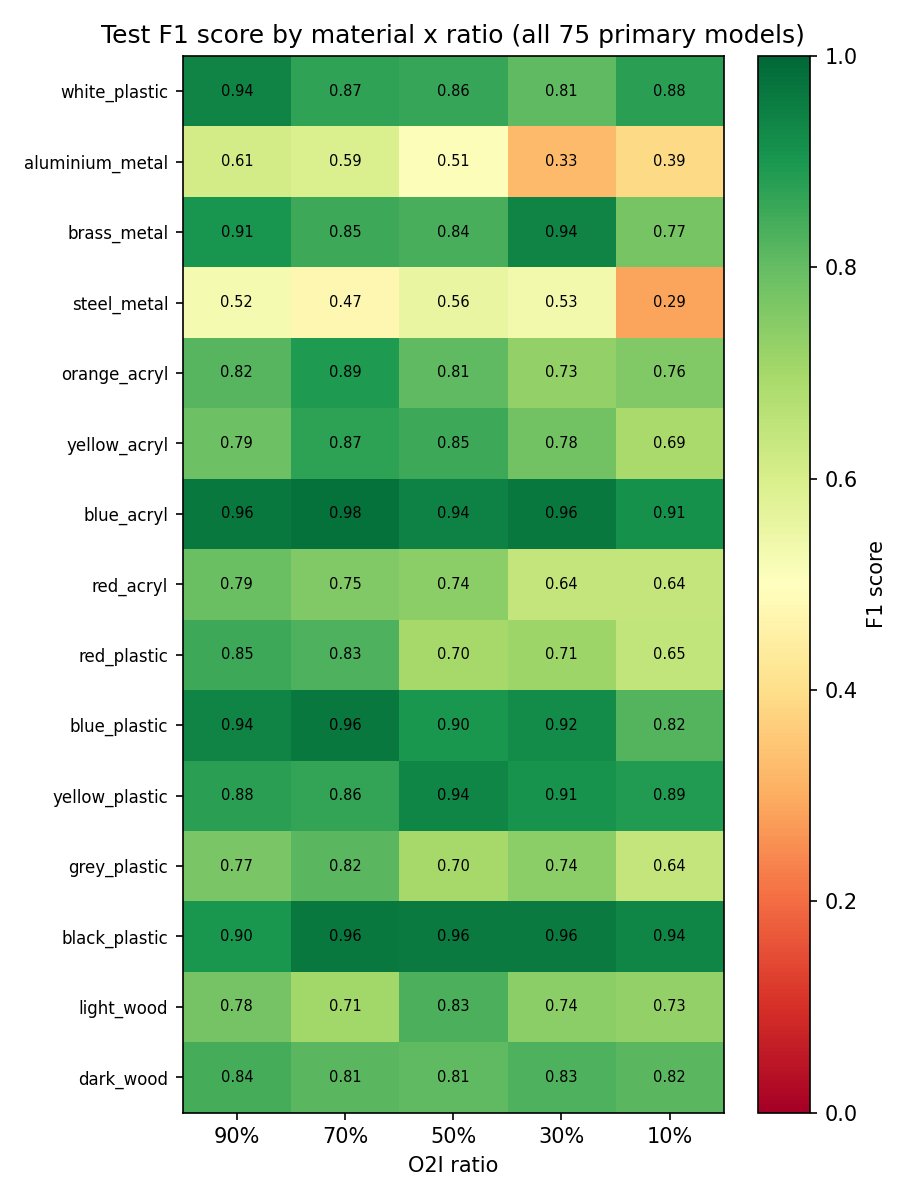
\includegraphics[width=0.6\textwidth]{fig_f1_heatmap.png}
\caption{The same 75 test F1 scores as Table~\ref{tab:ovr-full-results}, shown as a
material $\times$ ratio heatmap (green = high F1, red = low F1). The two metal rows
(aluminium, steel) stand out as a visibly weaker band across all five ratios, rather than
only at low ratios.}
\label{fig:f1-heatmap}
\end{figure}

Figure~\ref{fig:f1-per-material} makes visible a pattern the mean alone does not: the
decline is not uniform across materials. Several materials are almost flat across the
full ratio range -- black plastic stays between $0.90$ and $0.96$ F1 at every ratio, and
blue acryl between $0.91$ and $0.98$ -- while the two bare metals, aluminium and steel,
sit well below every other material at \emph{every} ratio, including $90\%$, where the
object fills most of the frame and background interference should, in principle, be
minimal. This is an important qualification of the headline ratio-decline finding: for
most materials, weak performance at low ratios is plausibly explained by background
dominance in the way the research question anticipates, but for aluminium and steel, poor
performance is already present when the object is large, which a pure O2I-ratio
explanation cannot account for on its own. Section~\ref{sec:results-qualitative}
investigates this anomaly directly using the occlusion sensitivity and Grad-CAM overlays,
and finds that the two metals fail for two genuinely different underlying reasons.

\subsection{Headline Finding: Occlusion Sensitivity and Grad-CAM Disagree}
\label{sec:results-divergence}

The explainability pipeline (Section~\ref{sec:methodology-explainability}) was run across
all 75 models, producing $750$ image analyses per method. Table~\ref{tab:centerfrac}
reports the mean $\text{center\_frac}$ (Section~\ref{sec:methodology-centerfrac}), averaged
across all 15 materials, at each of the five O2I ratios.

\begin{table}[h]
\centering
\begin{tabular}{lcc}
\hline
\textbf{O2I ratio} & \textbf{Occlusion sensitivity} & \textbf{Grad-CAM} \\
\hline
90\% & 0.556 & 0.709 \\
70\% & 0.582 & 0.657 \\
50\% & 0.612 & 0.672 \\
30\% & 0.661 & 0.627 \\
10\% & 0.721 & 0.407 \\
\hline
\end{tabular}
\caption{Mean $\text{center\_frac}$ by O2I ratio and explainability method, averaged
across all 15 materials (750 image analyses per method).}
\label{tab:centerfrac}
\end{table}

Grad-CAM shows the pattern the research question predicts: as the object shrinks from a
$90\%$ to a $10\%$ ratio, its $\text{center\_frac}$ falls from $0.709$ to $0.407$, meaning
the network's internal evidence increasingly originates outside the (shrinking) object
region as the background comes to dominate the frame. Occlusion sensitivity shows the
\emph{opposite} trend over the same range, rising from $0.556$ to $0.721$ -- reading as
\emph{more} object-focused, not less, precisely where Grad-CAM reads the model as
increasingly background-reliant. Both methods were applied to the same trained models on
the same sampled images, so this divergence is not attributable to a difference in what
was measured, only to how each method measures it.

This divergence is explained by a structural difference between the two methods rather
than by either one being faulty. Grad-CAM (Section~\ref{sec:background-gradcam}) computes
a single gradient over the \emph{entire} final feature map at once, so if the network
relies on the background as a whole -- not on any one specific spot, but on the general,
repeated presence of factory structure throughout the frame -- this holistic computation
is positioned to detect it. Occlusion sensitivity (Section~\ref{sec:background-occlusion}),
by contrast, is a strictly local, one-patch-at-a-time test. At a low O2I ratio, the object
occupies only a small region of the frame, so a single occluded patch can cover a large
fraction of the network's only concentrated positive evidence, producing a large,
easily-detected score change exactly at the object's location. The background, however, is
large and visually repetitive (the same conveyor, cables, and sensors recur throughout the
frame), so removing any \emph{one} patch of it leaves visually similar background fully
intact elsewhere in the image, and the measured effect of that single removal is small even
when the network genuinely depends on the background as a whole. Patch-based occlusion
sensitivity is therefore structurally insensitive to distributed reliance on redundant
background information, a limitation Grad-CAM does not share. This is developed further,
with reference to the wider explainability literature, in
Section~\ref{sec:discussion}.

\subsubsection{Qualitative Evidence: Occlusion and Grad-CAM Overlays}
\label{sec:results-qualitative}

Table~\ref{tab:centerfrac} reports the divergence between the two methods only as an
aggregate number, averaged over 750 images per method. To make this divergence concrete,
and to investigate the aluminium/steel anomaly surfaced in
Section~\ref{sec:results-primary-table}, this section examines individual occlusion
sensitivity and Grad-CAM overlays for three materials -- black plastic (the strongest,
most ratio-robust performer), and steel metal and aluminium metal (the two weakest
performers at every ratio) -- each shown at a $90\%$ and a $10\%$ O2I ratio. These are
illustrative single-image examples, not aggregate statistics, and are read accordingly:
they are used here to explain \emph{why} the aggregate numbers look the way they do, not
to replace them.

\begin{figure}[h]
\centering
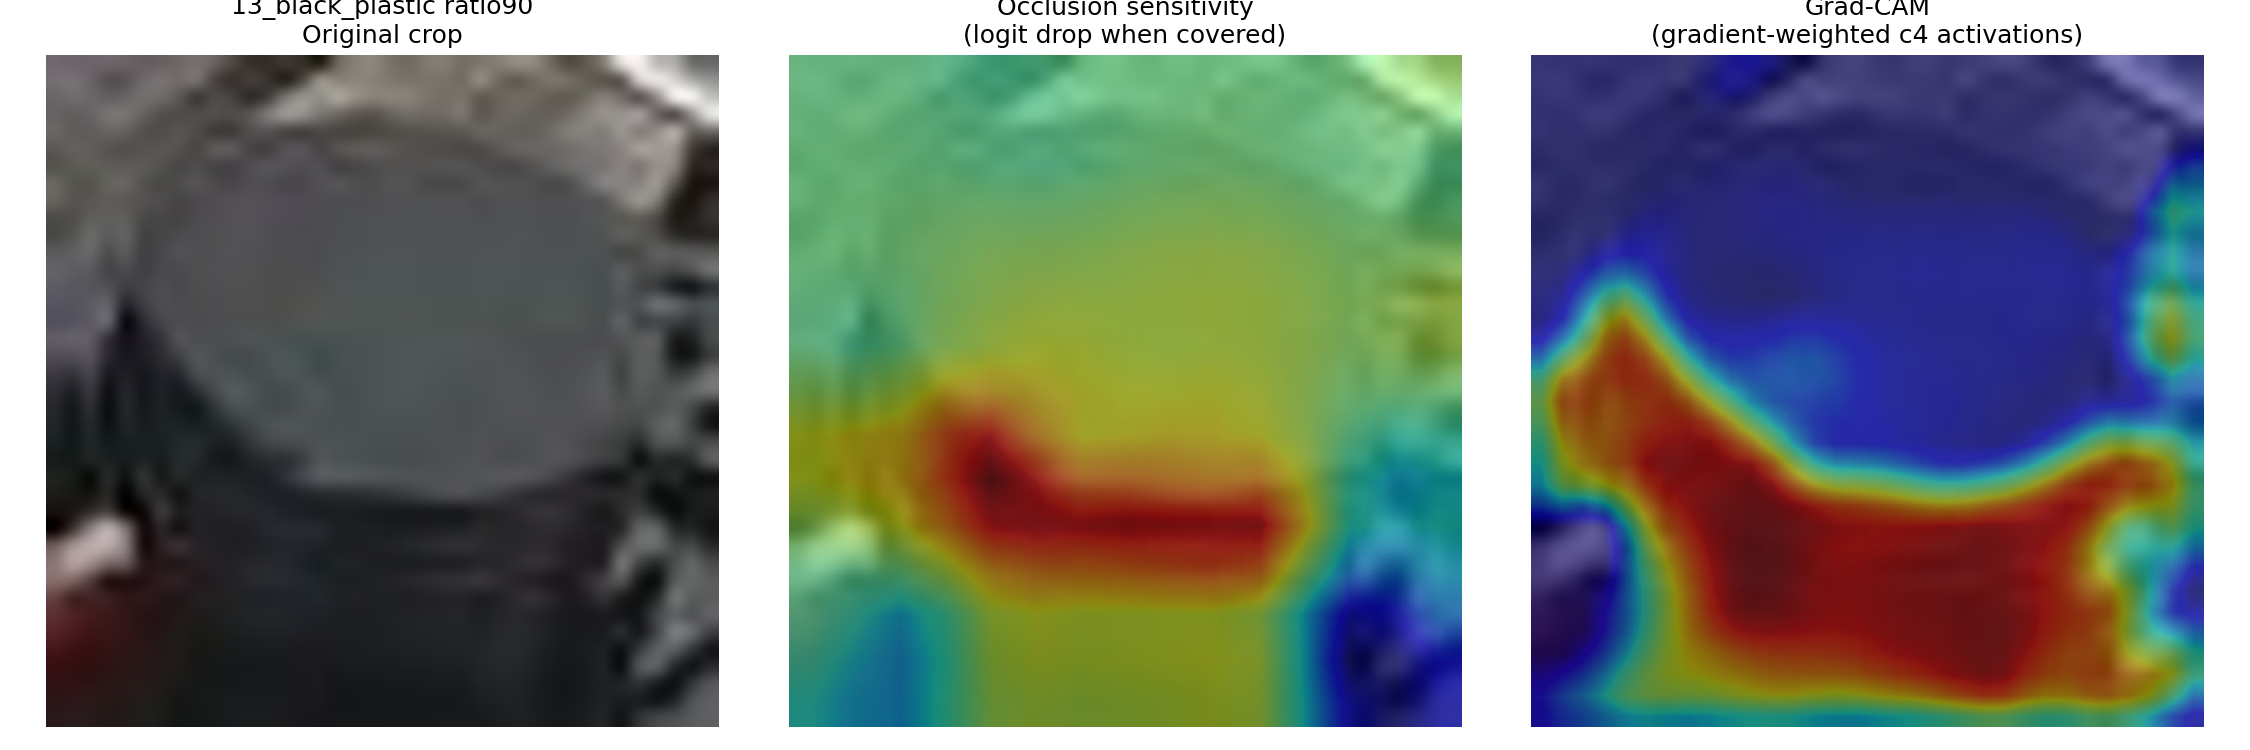
\includegraphics[width=\textwidth]{overlay_blackplastic_r90.png}
\caption{Black plastic, $90\%$ O2I ratio. Left: the original crop. Centre: occlusion
sensitivity (red = large logit drop when that patch is covered, i.e.\ the model relies on
it). Right: Grad-CAM (red = strong gradient-weighted activation). Both methods concentrate
on the same horizontal reflective highlight running across the workpiece's top surface --
a real, discriminative visual feature of this material's surface finish, not a background
artefact.}
\label{fig:overlay-black-r90}
\end{figure}

\begin{figure}[h]
\centering
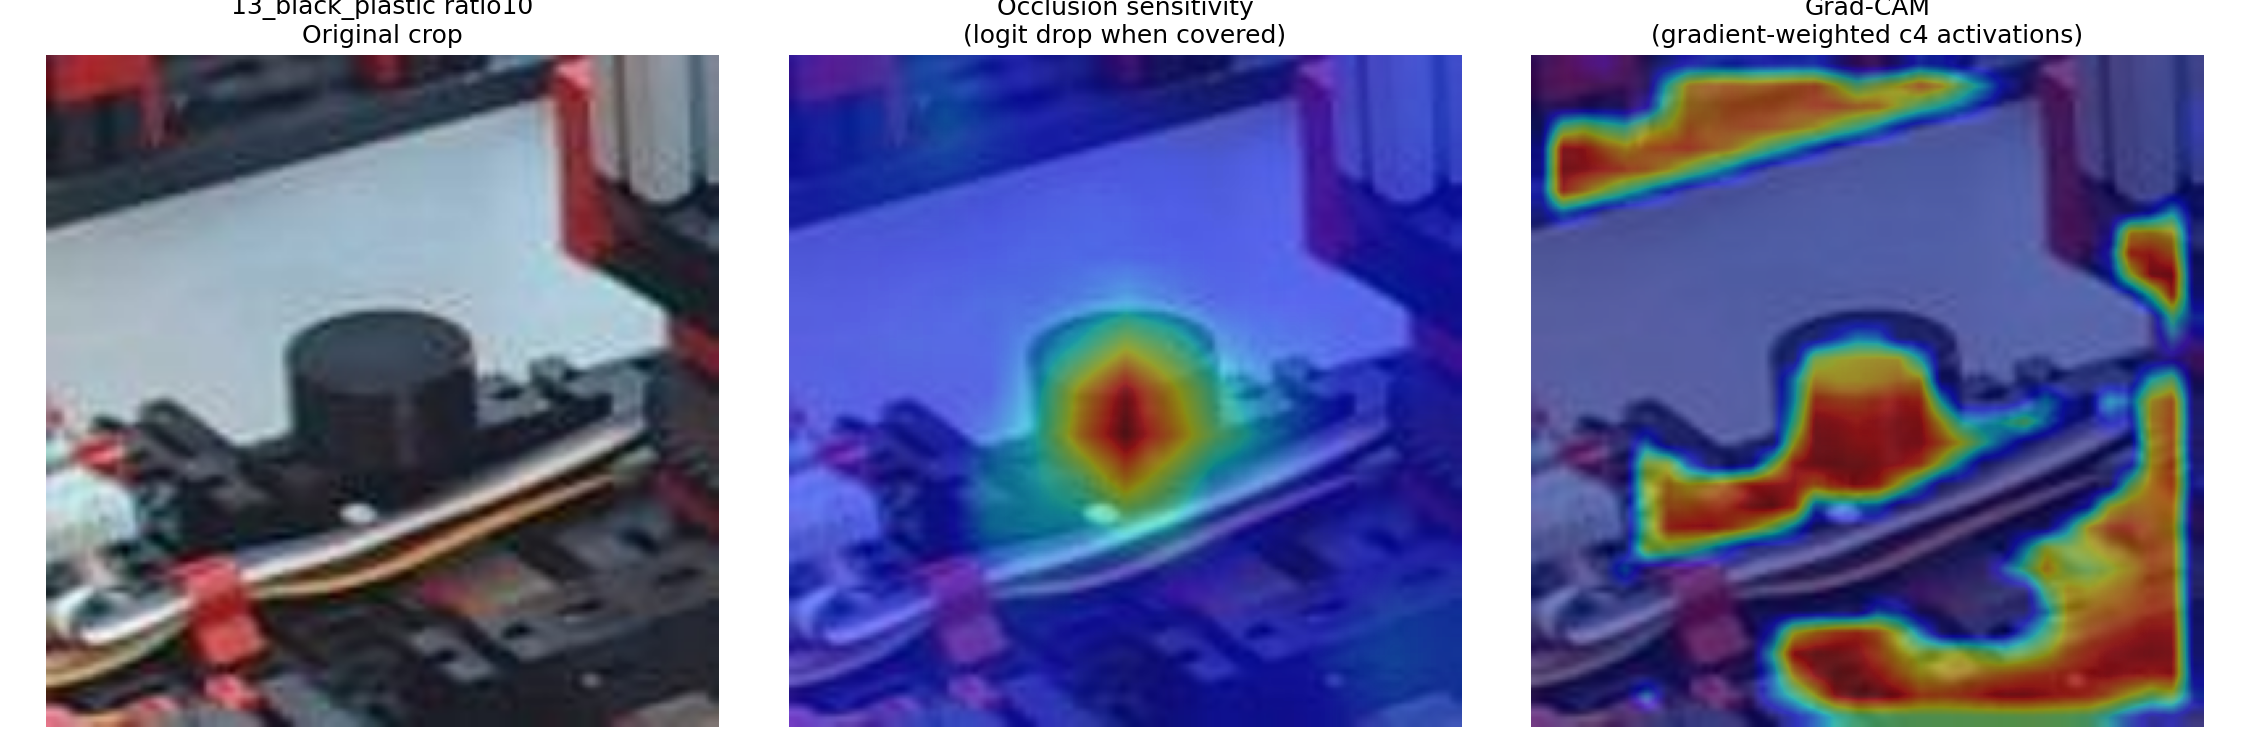
\includegraphics[width=\textwidth]{overlay_blackplastic_r10.png}
\caption{Black plastic, $10\%$ O2I ratio. Despite the object now occupying only a small
fraction of a visually busy frame (conveyor structure, metal brackets, another
workpiece), occlusion sensitivity forms a tight, sharply concentrated hotspot almost
exactly on the object, and Grad-CAM likewise concentrates its strongest activation on the
object and the bracket directly beneath it, with only minor spread into the surrounding
frame corners.}
\label{fig:overlay-black-r10}
\end{figure}

Black plastic's overlays are consistent with its near-flat F1 curve
(Figure~\ref{fig:f1-per-material}): even at a $10\%$ ratio, where background pixels
outnumber object pixels roughly nine to one, both explainability methods agree that the
network's decision is still substantially driven by the object itself. This is the
``well-behaved'' case the research question implicitly assumes as a baseline -- a material
whose visual signature is distinctive enough that the network continues to find and use
it even as the object shrinks.

\begin{figure}[h]
\centering
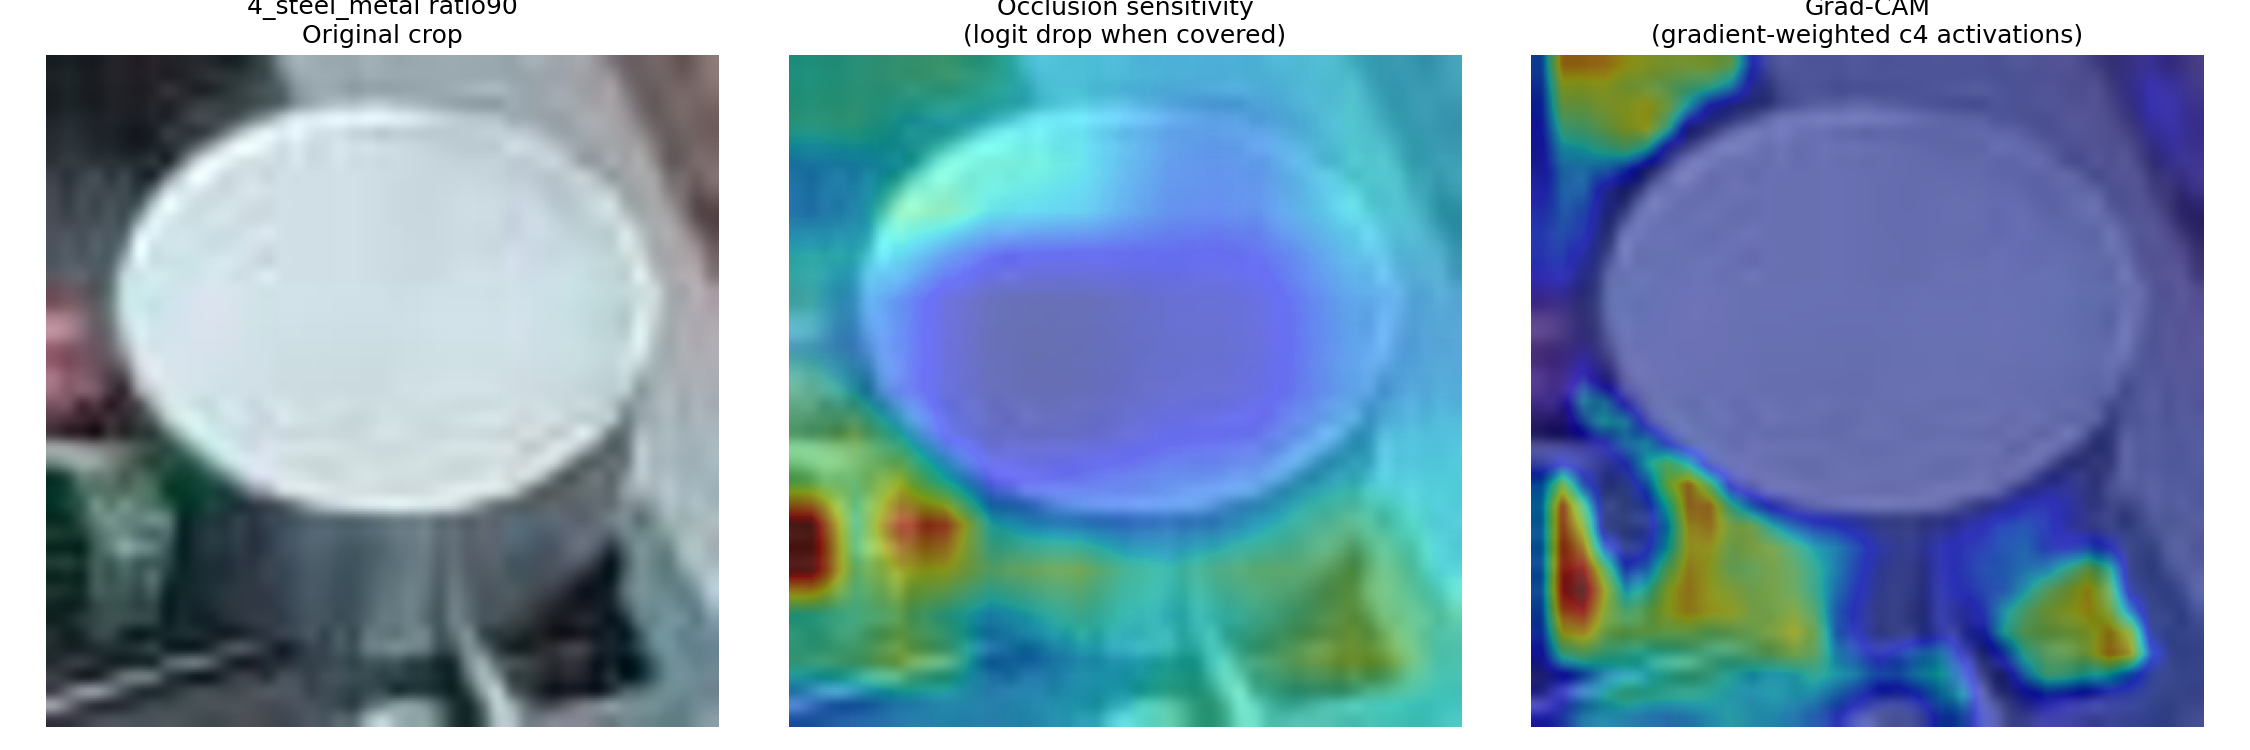
\includegraphics[width=\textwidth]{overlay_steelmetal_r90.png}
\caption{Steel metal, $90\%$ O2I ratio. The object fills most of the frame, yet both
occlusion sensitivity and Grad-CAM show only weak, near-neutral response \emph{on} the
object itself, with the strongest evidence in both maps located off the object, in the
background structure to its lower left.}
\label{fig:overlay-steel-r90}
\end{figure}

\begin{figure}[h]
\centering
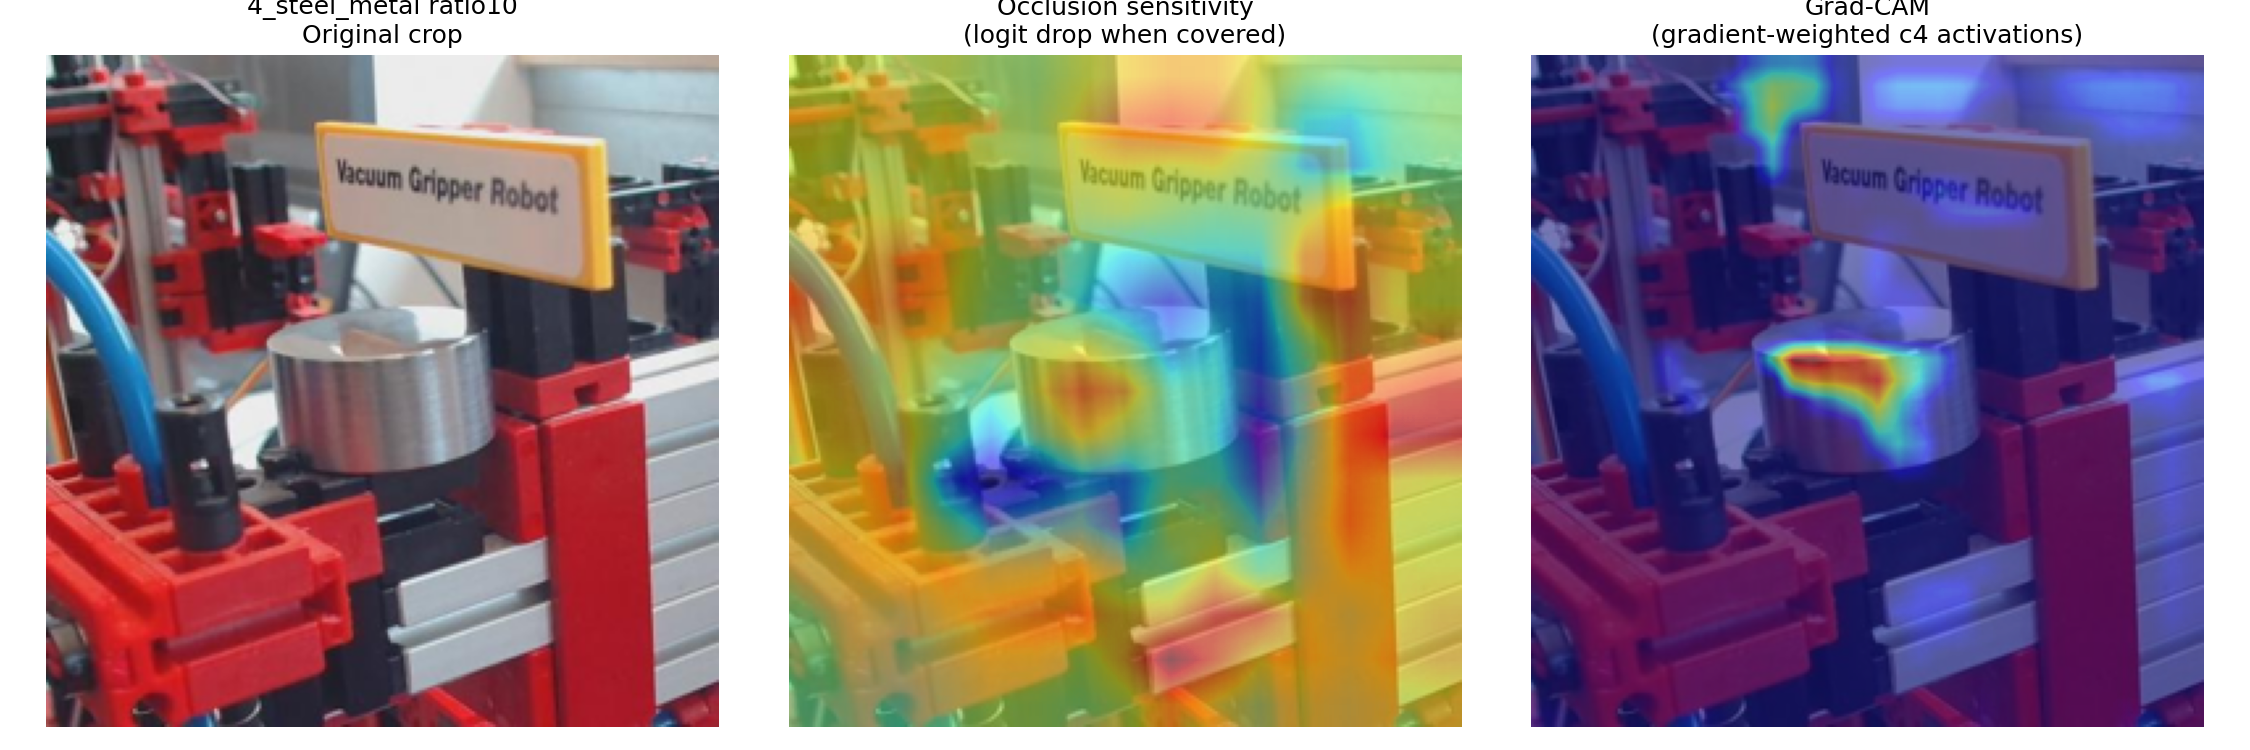
\includegraphics[width=\textwidth]{overlay_steelmetal_r10.png}
\caption{Steel metal, $10\%$ O2I ratio, in a scene containing the factory's ``Vacuum
Gripper Robot'' signage. Occlusion sensitivity is diffuse, spreading moderate sensitivity
broadly across much of the frame rather than concentrating sharply; Grad-CAM concentrates
more tightly on the object and the mechanism immediately beneath it.}
\label{fig:overlay-steel-r10}
\end{figure}

Steel metal's overlays explain why this material is the weakest performer in
Table~\ref{tab:ovr-full-results} at \emph{every} ratio, not only low ones.
Figure~\ref{fig:overlay-steel-r90} is the clearest single-image demonstration in this
thesis of background dominance occurring independently of the O2I ratio: with the object
occupying most of the frame, a pure ratio-driven account would predict strong,
object-centred evidence, but both methods instead point at the background. This suggests
that for steel, the factory background is not merely filling otherwise-empty space at low
ratios -- it is actively out-competing the object as a source of evidence even when the
object is large. A plausible physical explanation, consistent with steel's mirror-like,
highly reflective surface, is that the object's own surface appearance is partly a
reflection \emph{of} the surrounding factory environment, so the boundary between
``object'' and ``background'' information is less clean for this material than for a
matte plastic. Note, however, that Figure~\ref{fig:overlay-steel-r10} does not show a
simple continuation of this trend to an even more background-dominated state at the
lowest ratio -- if anything, Grad-CAM concentrates more on the object at $10\%$ than at
$90\%$ in this particular pair of sampled images. Given that each figure here is a single
illustrative example rather than an aggregate statistic, this should be read as a sign
that steel's failure mode is more complex than a monotonic ratio effect, not as evidence
against the aggregate trend in Table~\ref{tab:centerfrac}, which remains the statistically
supported result.

\begin{figure}[h]
\centering
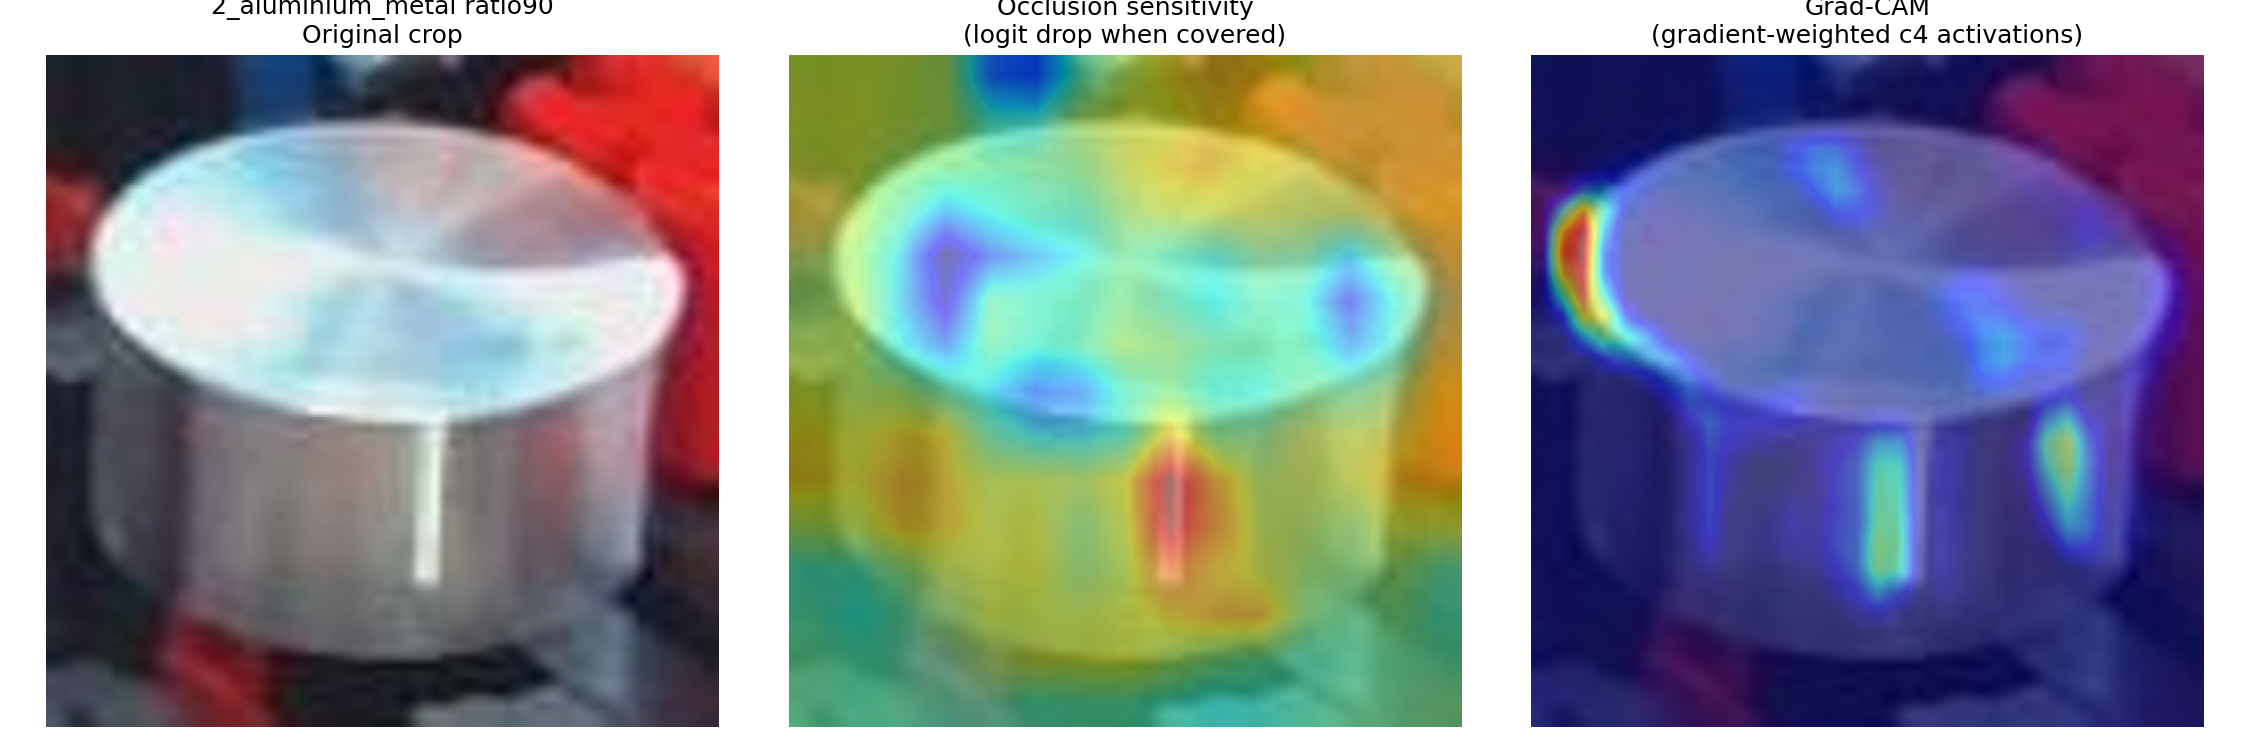
\includegraphics[width=\textwidth]{overlay_aluminiummetal_r90.png}
\caption{Aluminium metal, $90\%$ O2I ratio. Both methods concentrate mainly on or
immediately adjacent to the object -- its rim and a vertical reflective seam on its front
face -- with only modest spread into the neighbouring background structure, unlike the
steel case in Figure~\ref{fig:overlay-steel-r90}.}
\label{fig:overlay-alu-r90}
\end{figure}

\begin{figure}[h]
\centering
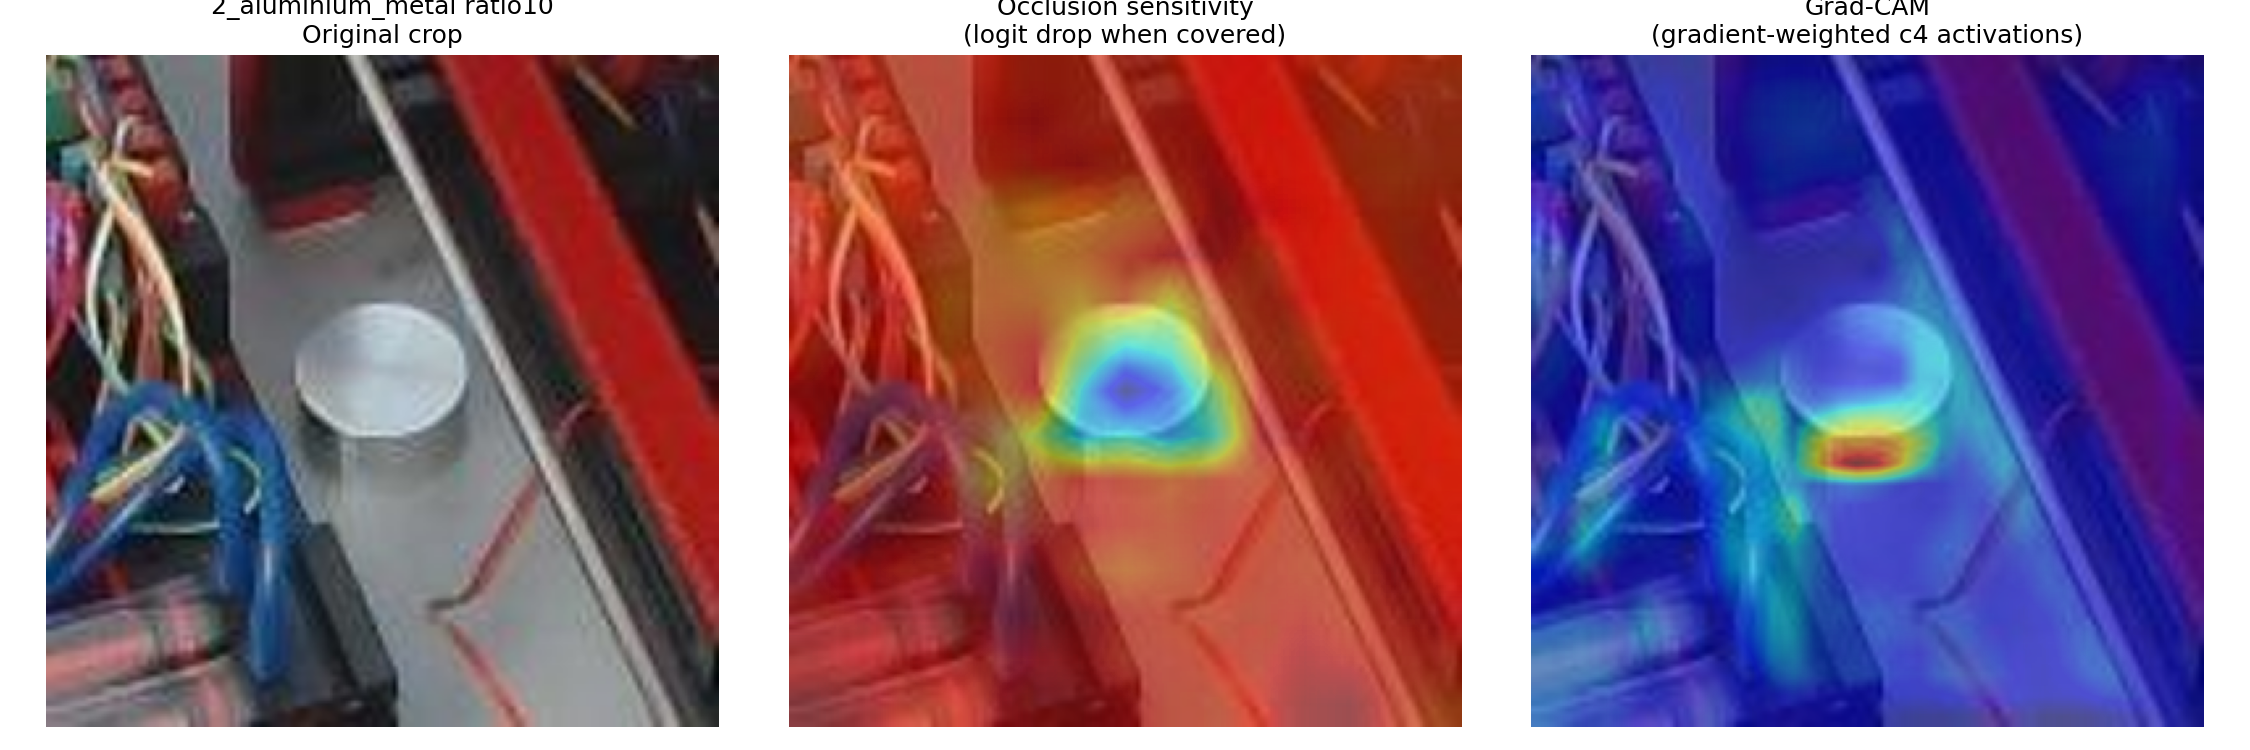
\includegraphics[width=\textwidth]{overlay_aluminiummetal_r10.png}
\caption{Aluminium metal, $10\%$ O2I ratio, amid factory wiring and conveyor rail. Both
methods form a hotspot essentially on the object itself, with only a small secondary
Grad-CAM response on the adjacent wire bundle.}
\label{fig:overlay-alu-r10}
\end{figure}

Aluminium metal is, by Table~\ref{tab:ovr-full-results}, almost as weak a performer as
steel (F1 between $0.33$ and $0.61$ across ratios), yet its overlays tell a visibly
different story: at both ratios shown, both explainability methods remain concentrated on
or very close to the object itself, not on the background. This is a genuinely useful
negative result: it shows that low F1 and background-focused attention are not the same
thing, and that the explainability pipeline can tell them apart. If aluminium's weak
classification were caused by background dominance in the way steel's appears to be, its
overlays should look like steel's; they do not. A more plausible explanation for
aluminium's weakness is instability in the object's \emph{own} visual signature rather
than reliance on the background: aluminium's polished surface reflects whatever
surrounds it (different conveyor sections, different lighting, nearby coloured parts),
so two aluminium crops can look quite different from each other even though the network
is correctly attending to the object in both. This would manifest as poor
material-versus-material discriminability despite good object localisation -- exactly
the pattern observed here. Steel and aluminium therefore illustrate two distinct failure
modes that happen to produce similarly poor F1 scores: steel's evidence-generation
apparatus reaches outside the object into the background, while aluminium's stays on the
object but the object's own appearance is an unreliable signal. Section~\ref{sec:discussion-material}
returns to this distinction.

\subsection{Robustness Checks}
\label{sec:results-robustness}

Before accepting the finding in Section~\ref{sec:results-divergence} as reliable, two
potential threats to its validity were investigated directly rather than assumed away.

\subsubsection{Grad-CAM Degeneracy}
\label{sec:results-degeneracy}

Grad-CAM is known to occasionally produce a completely flat, uninformative heatmap when
its ReLU step zeroes out every channel's contribution for a given image
(Section~\ref{sec:background-gradcam}). This occurred in $172$ of the $750$ analyses
($23\%$), with a strongly material-dependent rate: as low as $0\%$ for black plastic and
$2\%$ for brass metal and steel metal, but as high as $74\%$ for yellow plastic and over
$40\%$ for light wood, orange acryl, blue plastic, and grey plastic. Since a degenerate
heatmap falls back to the neutral $\text{center\_frac} = 0.5$
(Section~\ref{sec:methodology-centerfrac}), a concern is whether this degeneracy rate
could itself be manufacturing the downward Grad-CAM trend in Table~\ref{tab:centerfrac} --
for example, if degeneracy became more common at low ratios, pulling the mean toward the
neutral $0.5$ value in a way that mimicked a genuine shift toward the background. Checking
the degeneracy rate by ratio directly rules this out: $17\%$ (ratio 90), $27\%$ (ratio 70),
$17\%$ (ratio 50), $23\%$ (ratio 30), and $29\%$ (ratio 10) -- a mild increase at the
lowest ratio, but far too small and unevenly distributed across the middle ratios to
account for a shift from $0.709$ to $0.407$. The aggregate Grad-CAM trend in
Table~\ref{tab:centerfrac} is therefore not an artefact of degenerate heatmaps, though
per-material Grad-CAM results for the highest-degeneracy materials listed above should be
interpreted with this caveat in mind.

\subsubsection{Crop-Centering Validation}
\label{sec:results-centering}

The $\text{center\_frac}$ metric (Section~\ref{sec:methodology-centerfrac}) assumes the
object is centred within its crop; if this assumption failed, especially at low ratios
where the central box is small, the metric would be unreliable regardless of which
explainability method it is applied to. This was checked two ways: first, by reading the
crop-generation code directly, which crops symmetrically around the bounding-box centre
and therefore guarantees centering by construction rather than by approximation; second,
by directly measuring the object's pixel centroid on real sample crops, which confirmed an
offset of under $2\%$ of the crop dimension from true centre. The centering assumption
underlying $\text{center\_frac}$ is therefore confirmed to hold.

\subsection{Supplementary Investigation: Extended Training at 200 Epochs}
\label{sec:results-200epoch}

The primary results in this thesis use 100 training epochs
(Section~\ref{sec:methodology-training}). To check whether 100 epochs under-trained any
model, this investigation proceeded in two stages. First, three materials -- aluminium,
grey plastic, and steel metal -- were retrained for 200 epochs at all five O2I ratios (15
additional runs), chosen as an initial, quicker check spanning the primary results'
weakest performer (steel), a mid-table performer (grey plastic), and what turned out to be
the most severely undertrained material (aluminium). Table~\ref{tab:200epoch} reports this
first-stage result in detail, read row by row below, since walking through it concretely
motivated the second stage: extending the same check to the remaining 12 materials, which
Section~\ref{sec:results-200epoch-full} reports.

\begin{table}[h]
\centering
\footnotesize
\setlength{\tabcolsep}{4pt}
\begin{tabular}{p{2.1cm}cccccp{4cm}}
\hline
\textbf{Material} & \textbf{Ratio} & \textbf{F1@100} & \textbf{F1@200} & \textbf{Best ep.@200} & \textbf{$\Delta$} & \textbf{Interpretation} \\
\hline
Aluminium & 90\% & 0.588 & 0.698 & 168 & +0.110 & Large, genuine gain \\
Aluminium & 70\% & 0.597 & 0.756 & 198 & +0.159 & Large, genuine gain \\
Aluminium & 50\% & 0.615 & 0.741 & 159 & +0.126 & Large, genuine gain \\
Aluminium & 30\% & 0.432 & 0.607 & 197 & +0.175 & Largest gain; clearly undertrained at 100 \\
Aluminium & 10\% & 0.480 & 0.625 & 174 & +0.145 & Large, genuine gain \\
Grey plastic & 90\% & 0.824 & 0.857 & 147 & +0.033 & Moderate gain \\
Grey plastic & 70\% & 0.808 & 0.880 & 180 & +0.072 & Moderate gain \\
Grey plastic & 50\% & 0.808 & 0.830 & 194 & +0.022 & Small gain \\
Grey plastic & 30\% & 0.792 & 0.851 & 118 & +0.059 & Moderate gain \\
Grey plastic & 10\% & 0.723 & 0.829 & 199 & +0.106 & Large gain \\
Steel metal & 90\% & 0.702 & 0.700 & 161 & $\approx$0.000 & Flat; already converged \\
Steel metal & 70\% & 0.750 & 0.667 & 85 & $-$0.083 & Noisy outlier (see below) \\
Steel metal & 50\% & 0.702 & 0.735 & 130 & +0.033 & Moderate gain \\
Steel metal & 30\% & 0.632 & 0.652 & 182 & +0.021 & Small gain \\
Steel metal & 10\% & 0.480 & 0.564 & 173 & +0.084 & Moderate gain \\
\hline
\end{tabular}
\caption{200-epoch supplementary investigation. F1@100 is the original, once-recorded
baseline; F1@200 is the best F1 achieved across the full 200-epoch run; $\Delta$ is the
difference.}
\label{tab:200epoch}
\end{table}

Aluminium shows a large, consistent improvement at every ratio (+0.110 to +0.175),
indicating it was clearly undertrained at 100 epochs. Grey plastic shows a smaller but
still real and consistent improvement across all five ratios (+0.022 to +0.106). Steel
metal is not uniformly flat, contrary to an earlier, more limited observation based on
only two of its five ratios: ratio 90 shows no meaningful change, but ratios 50, 30, and 10
all show real, moderate gains, while ratio 70 shows an apparent \emph{drop}. This drop was
investigated rather than reported at face value: the ratio-70 rerun's own best F1 across
the \emph{entire} 200-epoch run occurred at epoch 85, before it had even reached epoch
100, and nothing in epochs 100--200 improved on it. This means the apparent drop is not a
case of additional training making the model worse (there is no overfitting-past-100
pattern in this run); rather, this particular training run underperformed the original run
from early on, most plausibly due to ordinary run-to-run numerical noise in GPU-based
training (e.g.\ from non-deterministic convolution algorithm selection) rather than any
systematic effect of extended training. It is reported here with this caveat explicit,
rather than as an unqualified $-0.083$ that would misleadingly suggest more training hurts
performance.

\subsubsection{Extending the Check to All 15 Materials}
\label{sec:results-200epoch-full}

The remaining 12 materials were subsequently retrained for 200 epochs at all five O2I
ratios as well (60 further runs), completing the check for the full primary result set.
Table~\ref{tab:200epoch-full} reports the resulting improvement, $\Delta = F1@200 -
F1@100$, for all 75 (material, ratio) combinations. A dagger ($\dagger$) marks a cell
where the 200-epoch run's own best F1 was reached before epoch 100 -- meaning that
particular run's peak occurred within what would have been the original 100-epoch window,
so its $\Delta$ cannot be attributed to the extra epochs at all and instead reflects
ordinary run-to-run training noise (the same situation already identified and explained
for steel metal at a $70\%$ ratio, immediately above). $19$ of the $75$ cells ($25\%$) are
flagged this way and are not over-interpreted individually.

\begin{table}[h]
\centering
\footnotesize
\setlength{\tabcolsep}{4pt}
\begin{tabular}{lccccc}
\hline
\textbf{Material} & \textbf{90\%} & \textbf{70\%} & \textbf{50\%} & \textbf{30\%} & \textbf{10\%} \\
\hline
White Plastic    & +0.017 & +0.000$^\dagger$ & +0.000$^\dagger$ & +0.041 & +0.000$^\dagger$ \\
Aluminium Metal  & +0.110 & +0.159 & +0.125 & +0.175 & +0.145 \\
Brass Metal      & +0.082$^\dagger$ & +0.040 & +0.000$^\dagger$ & +0.023 & +0.062 \\
Steel Metal      & -0.002 & -0.083$^\dagger$ & +0.033 & +0.021 & +0.084 \\
Orange Acryl     & +0.007$^\dagger$ & +0.010$^\dagger$ & +0.000$^\dagger$ & +0.016 & +0.020 \\
Yellow Acryl     & +0.105 & +0.000 & +0.019 & +0.026 & +0.099 \\
Blue Acryl       & +0.000$^\dagger$ & +0.000 & +0.000$^\dagger$ & +0.000$^\dagger$ & +0.021 \\
Red Acryl        & +0.016 & -0.013 & +0.008 & +0.027 & +0.033 \\
Red Plastic      & -0.016 & +0.038 & +0.092 & +0.007 & +0.000$^\dagger$ \\
Blue Plastic     & +0.019 & +0.018 & +0.000$^\dagger$ & +0.057 & +0.000$^\dagger$ \\
Yellow Plastic   & +0.036 & +0.038 & +0.041 & +0.020 & +0.023 \\
Grey Plastic     & +0.034 & +0.072 & +0.022 & +0.059 & +0.106 \\
Black Plastic    & +0.000$^\dagger$ & -0.020$^\dagger$ & +0.000$^\dagger$ & +0.000$^\dagger$ & +0.021 \\
Light Wood       & +0.027 & +0.058 & +0.032 & +0.073 & +0.042 \\
Dark Wood        & +0.032 & +0.005 & +0.048 & +0.018 & +0.048 \\
\hline
\textbf{Mean} & \textbf{+0.031} & \textbf{+0.022} & \textbf{+0.028} & \textbf{+0.037} & \textbf{+0.047} \\
\hline
\end{tabular}
\caption{$\Delta = F1@200 - F1@100$ for all 75 (material, ratio) combinations.
$^\dagger$~marks a cell where the 200-epoch run's own best epoch was below 100, so its
$\Delta$ reflects run-to-run noise rather than a genuine effect of extended training. The
bottom row is the mean $\Delta$ across all 15 materials at each ratio (including
noise-flagged cells, since their errors are as likely to understate as overstate the true
effect and should not be dropped from an average).}
\label{tab:200epoch-full}
\end{table}

Two things stand out. First, the per-material mean $\Delta$ (averaged across all five
ratios) ranks aluminium metal far above every other material at $+0.143$ -- more than
double the next-highest, grey plastic at $+0.059$ -- confirming that the pattern already
visible in the three-material check was not a coincidence of which materials happened to
be chosen first: aluminium is genuinely, substantially undertrained at 100 epochs, more so
than any other material in the study. Most materials cluster in a modest $+0.00$ to
$+0.05$ band (white plastic $+0.012$, blue acryl $+0.004$, orange acryl $+0.010$, black
plastic $+0.000$), indicating they were already close to converged at 100 epochs, which is
consistent with the healthy convergence behaviour observed directly in the loss curves for
most materials in Section~\ref{sec:results-convergence}.

Second, and directly relevant to the aluminium/steel discussion in
Section~\ref{sec:results-qualitative}: steel metal's own mean $\Delta$ is small, $+0.011$
-- close to the well-converged end of the range, not the undertrained end. This is an
important cross-check on that earlier qualitative finding. If steel's weak primary-result
F1 (Table~\ref{tab:ovr-full-results}) were simply an artefact of undertraining, extended
training should have closed much of the gap, the way it did for aluminium; instead, steel
gains almost nothing on average from doubling its training budget. This is independent,
quantitative support for the explanation offered in Section~\ref{sec:results-qualitative}
-- that steel's weakness reflects a genuine background-dominance effect visible in its
occlusion sensitivity and Grad-CAM overlays, not a model that simply needed more time to
train. Aluminium's own case is more nuanced: given its large mean $\Delta$, some of the
weak $100$-epoch F1 that motivated the qualitative analysis in
Section~\ref{sec:results-qualitative} does partly reflect undertraining rather than being
purely explained by an unstable, reflective object signal. However, this does not overturn
that analysis: checking directly, aluminium and steel remain the two lowest-F1 materials
in the entire study at \emph{every} O2I ratio even after 200 epochs of training
(F1@200 ranges $0.607$--$0.756$ for aluminium and $0.564$--$0.735$ for steel, both well
below the $0.76$--$1.00$ range nearly every other material occupies at 200 epochs). Extended
training narrows but does not close the gap between these two bare metals and the rest of
the dataset, so the qualitative distinction drawn between steel and aluminium's failure
modes in Section~\ref{sec:results-qualitative} is read as still standing, with the caveat
that aluminium's 100-epoch numbers specifically should be read as somewhat pessimistic
relative to what a fully-converged aluminium model would achieve.

% !TEX root = ../main.tex
\section{Discussion and Conclusion}
\label{sec:discussion}

This chapter answers the research question from the results of
Section~\ref{sec:results}, discusses the materials that depart from the average, and
closes with the limitations of the study, possible future work and a conclusion.

% ============================================================================
\subsection{Answering the Research Question}
\label{sec:discussion-answer}

The research question has two parts: at which O2I ratio the complex background of the
learning factory begins to dominate the classification decision, and whether
explainability methods can detect this shift. Section~\ref{sec:methodology-rq} sets out
how the results are read for each part, and the answer below follows that reading.

\paragraph{Classification}
Averaged over the 15 materials, the test F1 falls from 0.813 at an O2I ratio of 90\% to
0.720 at 10\% (Tab.~\ref{tab:ovr-full-results}), and it falls in 14 of the 15
materials. Most of this fall lies below 50\%. From 90\% to 50\% the mean changes by
$-0.017$, and the paired test shows no difference ($p = 0.25$), whereas from 50\% to
10\% it falls clearly, by 0.076 ($p = 0.001$). After 200 epochs the validation F1
still falls with the ratio, from 0.884 at 90\% to 0.841 at 10\%, against 0.854 to
0.794 after 100 epochs, so the training length explains a small part of the decline,
not the decline itself.

\paragraph{Two caveats}
The mean ROC-AUC stays between 0.970 and 0.982 at every ratio, so the models still rank
most positive crops above most negative ones while the F1 at the threshold $p_1 = 0.5$
falls. The decline of the F1 also does not isolate the background. With a fixed input
of $256 \times 256$ pixels, the side of a square with the area of the box shrinks from
about 243 pixels at 90\% to about 81 pixels at 10\%, i.e., from about 6.4 to about 2.1
times the 38-pixel receptive field of the fourth convolutional layer (paragraph
\emph{What changes with the ratio} in Section~\ref{sec:methodology-crops}). The F1
decline fits a growing influence of the background, but it cannot separate that
influence from the smaller scale of the workpiece.

\paragraph{Where the evidence lies}
The Grad-CAM centre measure falls at every step, from 0.737 at 90\% to 0.407 at 10\%
(Tab.~\ref{tab:centerfrac}). At these mean values, Eq.~\eqref{eq:odds} gives
$m_{\mathrm{in}}/m_{\mathrm{out}} = 2.80$ and 0.69. Since every reference value rises as
the ratio falls (Tab.~\ref{tab:reference}), the fall can come neither from the geometry
of the square nor from the resolution of Grad-CAM, and it is read as evidence moving
from the workpiece into the background. Its largest step, from 30\% to 10\%, lies in
the same interval as the largest step of the F1. This is a description of the two
curves, not a tested result (Section~\ref{sec:methodology-tests}).

Under the rule of Section~\ref{sec:methodology-rq}, the background outweighs the
workpiece only where $c$ lies clearly below 0.5, and this holds at no ratio for either
method. At 10\%, Grad-CAM is below 0.5 on average and in 9 of the 15 materials, but not
clearly ($t(14) = -1.36$), and the same holds without the flat maps (0.363,
$t(14) = -1.64$). The criterion is strict by design. At 10\% the region outside the
reference square has about nine times its area, so the background holds more of the
total importance whenever $c$ is below about 0.9. By that total, even occlusion would
show the background dominating at 10\% on average, since its mean centre measure of
0.884 lies below 0.9 although it strongly favours the square per pixel. The total depends on the area of
the square and would change with the ratio even for a flat map, which is why the
per-pixel measure is used (Section~\ref{sec:methodology-rq}). The answer to the first
part of the research question is therefore a gradual shift of the evidence towards the
background over the five ratios, without a ratio at which the background clearly
dominates, although the classification suffers mainly below 50\%.

\paragraph{Detection of the shift}
By the detection rule of Section~\ref{sec:methodology-rq}, Grad-CAM detects the shift:
its centre measure changes by $-0.330$ from 90\% to 10\% ($t(14) = -4.17$) while the
test F1 changes by $-0.093$ ($t(14) = -4.76$). Occlusion sensitivity does not, since
its centre measure rises from 0.728 to 0.884. The rise does not show that the occlusion
evidence stays on the workpiece. The occlusion reference value rises faster, from 0.569
to 0.956, so the reference gap of occlusion falls from $+0.159$ at 90\% to about zero or
below from 50\% on. This fall is at most an indirect sign of a shift, since the
reference gaps are not tested as trends (Section~\ref{sec:methodology-refgap}).

The two methods agree at 90\% and then move apart. The method difference is clear at
10\% (0.477) and as a slope over the five ratios, and at 10\% the difference beyond the
reference is 0.509, so the different resolutions of the two methods do not produce it
(Section~\ref{sec:results-reference}). Grad-CAM thus detects the shift and occlusion
sensitivity, the method specified for this thesis, does not, and whether a shift of the
evidence is visible depends on the method used to look for it. None of the five checks of
Section~\ref{sec:results-robustness} changes this result. The agreement at 90\% does
not hold under all of them: it holds only for positive drops with the grey fill, while
with min-max normalisation or a blurred patch occlusion lies clearly below Grad-CAM at
90\%.

\paragraph{Why the two methods answer differently}
Section~\ref{sec:background-comparison} gives the reason why the two methods can
disagree. If the background holds many similar cues, like a room full of clocks,
covering one of them with a patch changes the score little, while Grad-CAM marks all of
them at once. The results add two points to this. At 10\% the workpiece fits into a
reference square of about 81 pixels, and one $32 \times 32$ patch covers about 40\% of
its width, so a few patches remove most of the workpiece and the drops concentrate
there. Together with the rising reference value, this would explain why the occlusion
centre measure even rises as the ratio falls. The fill of the patch, in contrast, cannot
explain the average divergence, since the divergence appears with the grey, the black
and the blurred patch alike (Section~\ref{sec:results-fill}); the fill matters for
single workpieces (Section~\ref{sec:discussion-material}). The redundancy explanation
remains a hypothesis. The thesis measures that the methods diverge, not why. The toy of
Section~\ref{sec:background-comparison} shows only the ingredients, and neither map is
ground truth for what the model uses. A direct test would replace the whole background
at once instead of one patch (Section~\ref{sec:discussion-future}).

\paragraph{On average, not per material}
The detection rule compares means over the 15 materials. It shows that the mean F1 and
the mean Grad-CAM centre measure fall together, not that the materials whose
classification suffers most are those whose evidence moves most, and per material no
such link is shown. Over the 15 materials, the change from 90\% to 10\% of the test F1
(Tab.~\ref{tab:ovr-full-results}) and that of the per-model Grad-CAM centre measures
behind Tab.~\ref{tab:centerfrac} give a Pearson correlation of $r = -0.20$
($p = 0.47$) and a Spearman rank correlation of $\rho = -0.14$ ($p = 0.63$). Steel
loses most F1, 0.230, while its Grad-CAM centre measure rises by 0.148, aluminium loses
0.224 while its centre measure falls by only 0.074, and blue AG has the largest
Grad-CAM fall, 0.827, with almost no loss of F1 (0.028). Grad-CAM thus shows that the
evidence shifts towards the background as the background grows, not that this shift is
why a given material is misclassified (Section~\ref{sec:discussion-material}).

\paragraph{Relation to earlier work}
The gradual decline of the F1, without a fall to chance, fits the results of Pawlowski
et al.~\cite{pawlowski2019needles} for ratio ranges that cover those studied here
(Section~\ref{sec:related-work-o2i}). Unlike their saliency maps, which fail where the
classifier fails, the Grad-CAM evidence here moves away from the workpiece while the
classification declines only moderately and the models still rank the crops well
(mean ROC-AUC of at least 0.970). Xiao et al.~\cite{xiao2021noise} showed that the
background can carry evidence for a class, so evidence in the background is not by
itself an error. Their further finding, that more accurate models exploit the
background more, compares different architectures on the same images, whereas here one
architecture is trained on crops of different ratios.

% ============================================================================
\subsection{Material-Dependent Effects}
\label{sec:discussion-material}

[6.2 to follow]

% ============================================================================
\subsection{Limitations}
\label{sec:discussion-limitations}

[6.3 to follow]

% ============================================================================
\subsection{Future Work}
\label{sec:discussion-future}

[6.4 to follow]

% ============================================================================
\subsection{Conclusion}
\label{sec:discussion-conclusion}

[6.5 to follow]


% -------------------- BIBLIOGRAPHY --------------------
\bibliographystyle{plainnat}
\bibliography{references}

\end{document}
